\section{Model Description}

\subsection{Problem Statement}

The formulation assumes that there is a rigid hub, with $N_P$ lumped masses in the tank for the fuel. Subscript $j$ is used to indicate the $j_\text{th}$ fuel slosh mass, $m_j$. Figure~\ref{fig:Slosh_Figure} displays the frame and variable definitions used for this formulation.

\begin{figure}[ht]
	\centering
	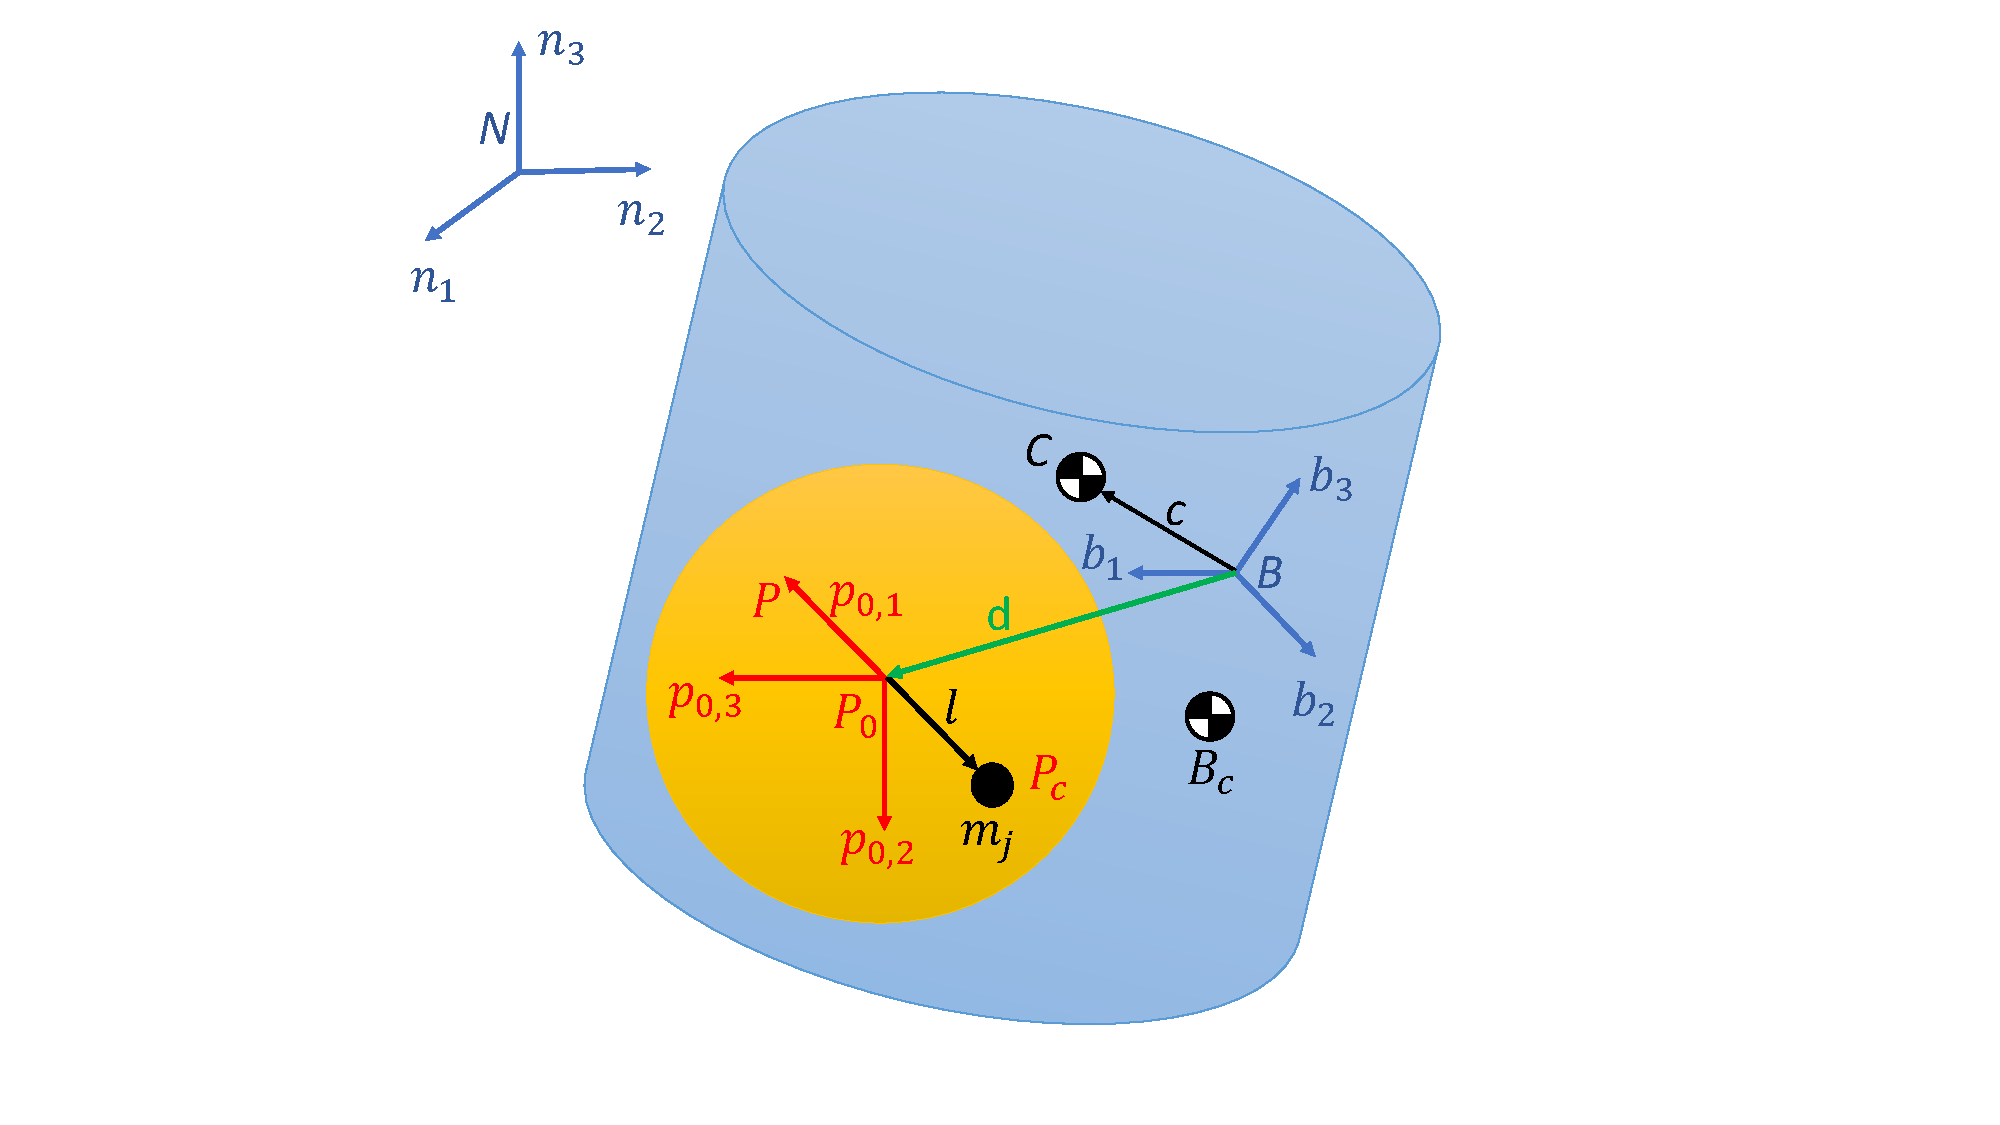
\includegraphics[width=13cm]{Figures/spacecraft.pdf}
	\caption{Frame and variable definitions used for formulation}
	\label{fig:Slosh_Figure}
\end{figure} 

There are four coordinate frames defined for this formulation. The inertial reference frame is indicated by \frameDefinition{N}. The body fixed coordinate frame, \frameDefinition{B}, which is anchored to the hub and can be oriented in any direction. The initial pendulum frame, $\mathcal{P}_{0,j}:\{\hat{\bm p}_{0_j,1},\hat{\bm p}_{0_j,2},\hat{\bm p}_{0_j,3}\}$, is a frame with its origin located at tank geometrical center, $T$. The $\mathcal{P}_{0,j}$ frame is a fixed frame respect to the body frame, oriented such that $\hat{\bm{p}}_{0_j,1}$ points to the fuel slosh mass in its initial position, $P_{j}$. The constant distance from point $T$ to point $P_{j}$ is defined as $l_j$. 

There are a few more key locations that need to be defined. Point $B$ is the origin of the body frame, and can have any location with respect to the hub. Point $B_c$ is the location of the center of mass of the rigid hub. $P_{c,j}$ is the instantaneous position of the fuel slosh mass $m_j$. $\bm{d}$ is vector from the center of the body reference system to the tank geometrical center. $\bm{l_j}$ is the vector from $T$ to $P_{c,j}$.

Figure~\ref{fig:Slosh_Detailed} provides further detail of the fuel slosh parameters and reference frames. As seen in Figure~\ref{fig:Slosh_Figure}, an individual slosh particle is free to move in every direction while connected by rigid weightless rod to the geometrical center of the tank. A linear damper effect is considered using a damping matrix, $D$. The variables, $\varphi_j$ and $\vartheta_j$ are state variables and quantify the angular displacement from initial position for the corresponding slosh mass. 

\begin{figure}[ht]
	\centering
	
	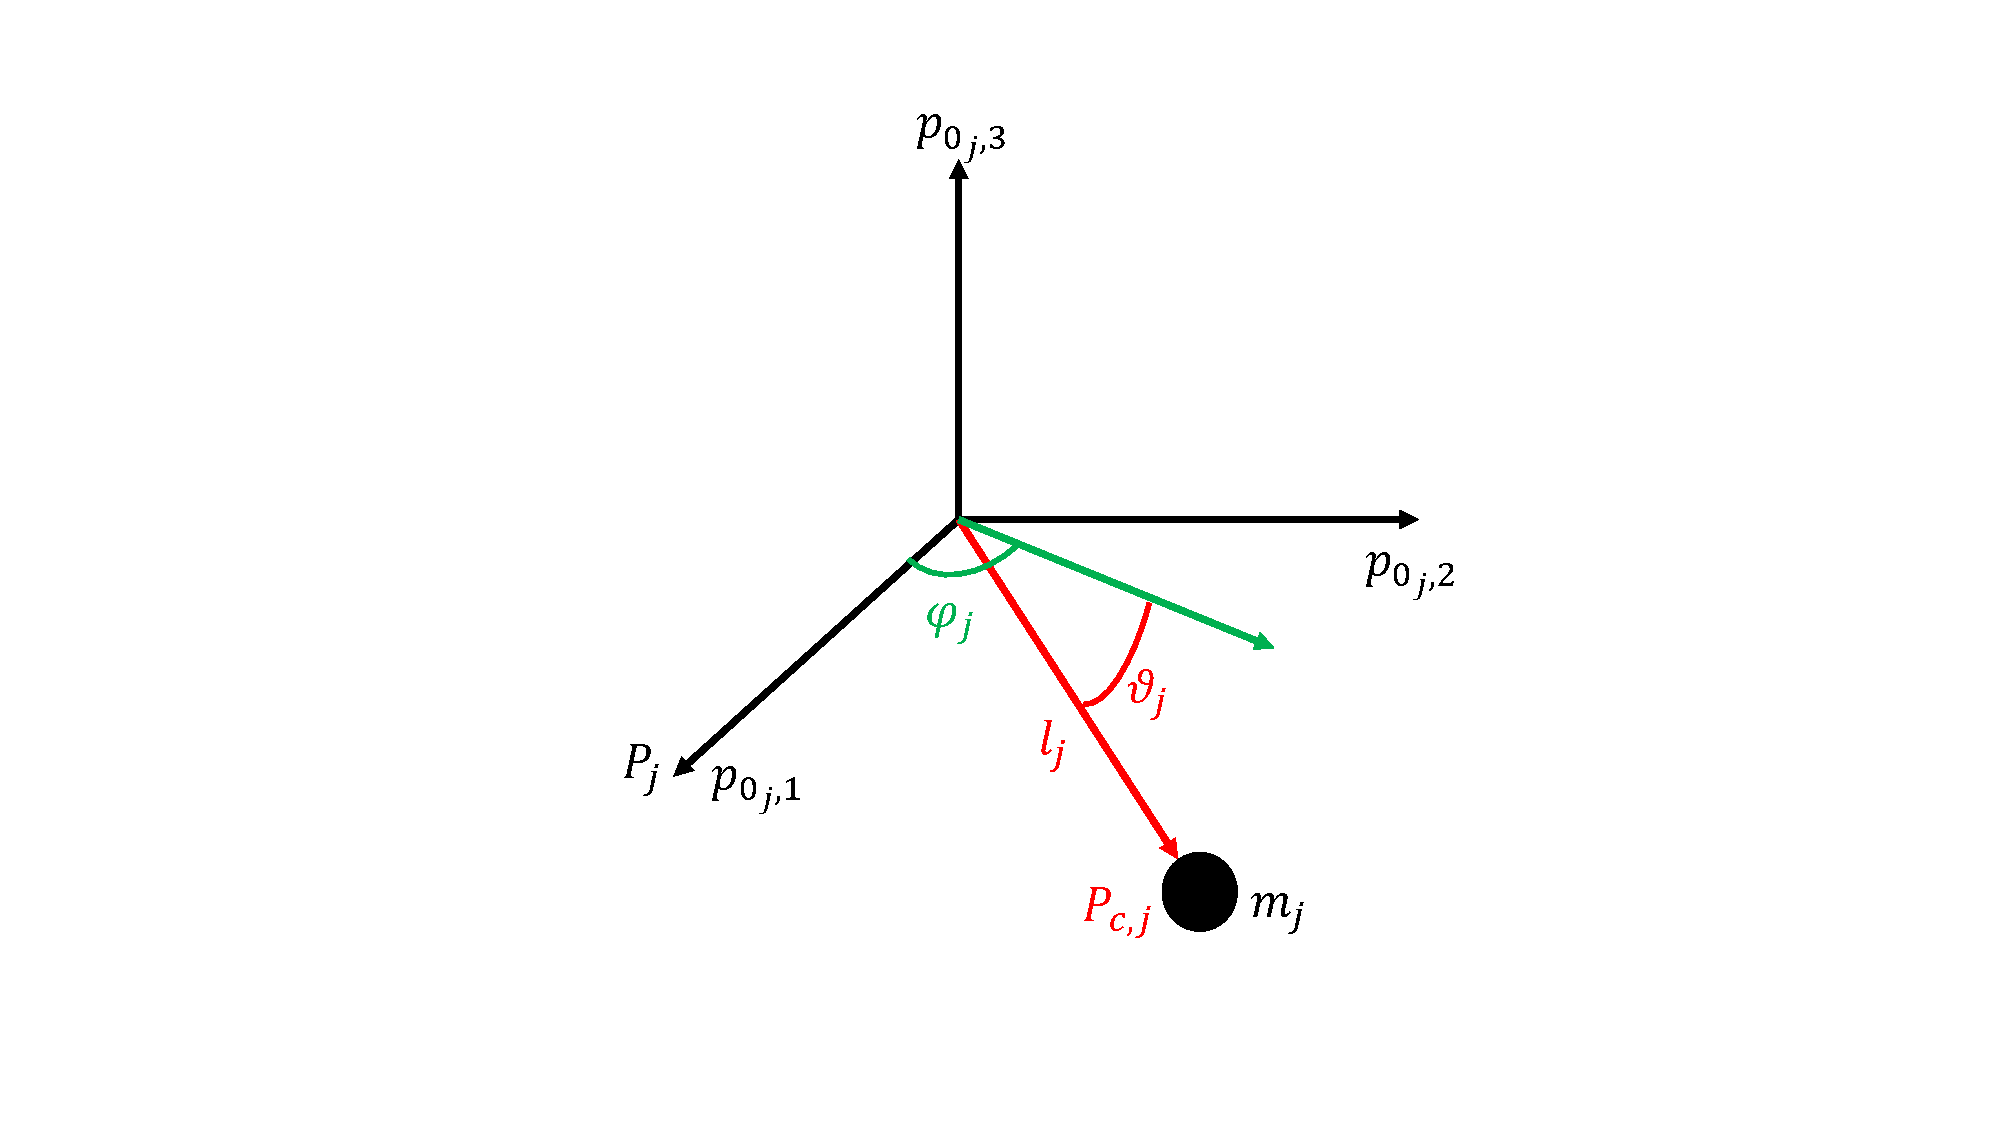
\includegraphics[width=13cm]{Figures/referencesystems.pdf}
	\caption{Further detail of fuel slosh and reference frames}
	\label{fig:Slosh_Detailed}
\end{figure}

Using the variables and frames defined, the following section outlines the derivation of equations of motion for the spacecraft.

\subsection{Derivation of Equations of Motion}

\subsubsection{Rigid Spacecraft Hub Translational Motion}

The derivation begins with Newton's first law for the center of mass of the spacecraft.
\begin{equation}
	\ddot{\bm r}_{C/N} = \frac{\bm{F}}{m_{\text{\text{sc}}}}
	\label{eq:Newtons1Law}
\end{equation}
Ultimately the acceleration of the body frame or point $B$ is desired
\begin{equation}
	\ddot{\bm r}_{B/N} = \ddot{\bm r}_{C/N}-\ddot{\bm c}
	\label{eq:RcRbacc}
\end{equation}
The definition of $\bm{c}$ can be seen in Eq. (\ref{eq:c}).
\begin{equation}
	\bm{c} = \frac{1}{m_{\text{sc}}}\Big(m_{\text{\text{hub}}}\bm{r}_{B_{c}/B} +\sum_{j=1}^{N_{P}}m_j\bm{r}_{P_{c,j}/B}\Big)
	\label{eq:c} 
\end{equation}
To find the inertial time derivative of $\bm{c}$, it is first necessary to find the time derivative of $\bm{c}$ with respect to the body frame. A time derivative of any vector, $\bm{v}$, with respect to the body frame is denoted by $\bm{v}'$; the inertial time derivative is labeled as $\dot{\bm{v}}$. The first and second body-relative time derivatives of $\bm{c}$ can be seen in Eqs. (\ref{eq:cprime}) and (\ref{eq:cdprime}).
\begin{align}
	\bm{c}' &= \frac{1}{m_{\text{sc}}}\Big(\sum_{j=1}^{N_{P}}m_j\bm{r}'_{P_{c,j}/B}\Big)
	\label{eq:cprime}
	\\
	\bm{c}'' &= \frac{1}{m_{\text{sc}}}\Big(\sum_{j=1}^{N_{P}}m_j\bm{r}''_{P_{c,j}/B}\Big)
	\label{eq:cdprime}
\end{align}
Remembering that the derivative of $d$ is null respect to the body frame, the first and second body time derivatives of $\bm{r}_{P_{c,j}/B}$ are
\begin{equation}
	\bm{r}_{P_{c,j}/B} = 
	l_j
	\leftidx{^{\mathcal{P}_{0,j}}}
	{\begin{bmatrix}
			\cos(\varphi_j)\cos(\vartheta_j) \\
			\sin(\varphi_j)\cos(\vartheta_j) \\
			-\sin(\vartheta_j)
	\end{bmatrix}}
	+ d
	\label{eq:rPcjB}
\end{equation}

\begin{equation}
	\bm{r}'_{P_{c,j}/B} 
	=
	l_j 
	\leftidx{^{\mathcal{P}_{0,j}}}
	{\begin{bmatrix}
			-\dot{\varphi}_j\sin(\varphi_j)\cos(\vartheta_j)-\dot{\vartheta}_j\cos(\varphi_j)\sin(\vartheta_j) \\
			\dot{\varphi}_j\cos(\varphi_j)\cos(\vartheta_j)-\dot{\vartheta}_j\sin(\varphi_j)\sin(\vartheta_j) \\
			-\dot{\vartheta}_j\cos(\vartheta_j)
	\end{bmatrix}}
	\label{eq:rPcjBprime}
\end{equation}

\begin{equation}
	\bm{r}''_{P_{c,j}/B} 
	=
	l_j
	\leftidx{^{\mathcal{P}_{0,j}}}
	{\begin{bmatrix}
			-\ddot{\varphi}_j\sin(\varphi_j)\cos(\vartheta_j)-\ddot{\vartheta}_j\cos(\varphi_j)\sin(\vartheta_j)-\dot{\varphi}_j^2\cos(\varphi_j)\cos(\vartheta_j)\\-\dot{\vartheta}_j^2\cos(\varphi_j)\cos(\vartheta_j)+2\dot{\varphi}_j\dot{\vartheta}_j\sin(\varphi_j)\sin(\vartheta_j) \\ \\
			\ddot{\varphi}_j\cos(\varphi_j)\cos(\vartheta_j)-\ddot{\vartheta}_j\sin(\varphi_j)\sin(\vartheta_j)-\dot{\varphi}_j^2\sin(\varphi_j)\cos(\vartheta_j)\\-\dot{\vartheta}_j^2\sin(\varphi_j)\cos(\vartheta_j)-2\dot{\varphi}_j\dot{\vartheta}_j\cos(\varphi_j)\sin(\vartheta_j) \\ \\
			-\ddot{\vartheta}_j\cos(\vartheta_j)+\dot{\vartheta}_j^2\sin(\vartheta_j)
	\end{bmatrix}}
	\label{eq:rPcjBprimeprime}
\end{equation}
Eqs.~\eqref{eq:cprime} and ~\eqref{eq:cdprime} are next reformulated to include these new definitions:


\begin{multline}
	\bm{c}' = \frac{1}{m_{\text{sc}}}\sum_{j=1}^{N_{P}}m_j l_j \bigg[\Big(-\dot{\varphi}_j\sin(\varphi_j)\cos(\vartheta_j)-\dot{\vartheta}_j\cos(\varphi_j)\sin(\vartheta_j)\Big)\bm{\hat{p}}_{0_j,1}+\\
	\Big(\dot{\varphi}_j\cos(\varphi_j)\cos(\vartheta_j)-\dot{\vartheta}_j\sin(\varphi_j)\sin(\vartheta_j) \Big)\bm{\hat{p}}_{0_j,2}  -\dot{\vartheta}_j\cos(\vartheta_j) \bm{\hat{p}}_{0_j,3} \bigg]
	\label{eq:cprime2}
\end{multline}


\begin{multline}
	\bm{c}'' = \frac{1}{m_{\text{sc}}}\sum_{j=1}^{N_{P}}m_j l_j \bigg[
	\Big(-\ddot{\varphi}_j\sin(\varphi_j)\cos(\vartheta_j)-\ddot{\vartheta}_j\cos(\varphi_j)\sin(\vartheta_j)-\dot{\varphi}_j^2\cos(\varphi_j)\cos(\vartheta_j)-\dot{\vartheta}_j^2\cos(\varphi_j)\cos(\vartheta_j)\\+2\dot{\varphi}_j\dot{\vartheta}_j\sin(\varphi_j)\sin(\vartheta_j) \Big)\bm{\hat{p}}_{0_j,1} 
	+\Big(\ddot{\varphi}_j\cos(\varphi_j)\cos(\vartheta_j)-\ddot{\vartheta}_j\sin(\varphi_j)\sin(\vartheta_j)-\dot{\varphi}_j^2\sin(\varphi_j)\cos(\vartheta_j)\\-\dot{\vartheta}_j^2\sin(\varphi_j)\cos(\vartheta_j)-2\dot{\varphi}_j\dot{\vartheta}_j\cos(\varphi_j)\sin(\vartheta_j) \Big)\bm{\hat{p}}_{0_j,2}
	+\Big(-\ddot{\vartheta}_j\cos(\vartheta_j)+\dot{\vartheta}_j^2\sin(\vartheta_j) \Big)\bm{\hat{p}}_{0_j,3}
	\bigg]
	\label{eq:cdprime2}
\end{multline}
Using the transport theorem yields the following definition for $\ddot{\bm c}$
\begin{equation}
	\ddot{\bm c} = \bm{c}'' + 2\bm\omega_{\cal B/N}\times\bm{c}'+\dot{\bm\omega}_{\cal B/N}\times\bm{c}+\bm\omega_{\cal B/N}\times\left(\bm\omega_{\cal B/N}\times\bm{c}\right)
	\label{eq:cddot}
\end{equation}
Eq.~\eqref{eq:RcRbacc} is updated to include Eq.~\eqref{eq:cddot}

\begin{equation}
	\ddot{\bm r}_{B/N} = \ddot{\bm r}_{C/N}-\bm{c}'' - 2\bm\omega_{\cal B/N}\times\bm{c}'-\dot{\bm\omega}_{\cal B/N}\times\bm{c}-\bm\omega_{\cal B/N}\times\left(\bm\omega_{\cal B/N}\times\bm{c}\right)
	\label{eq:Rbddot}
\end{equation}
Substituting Eq.\eqref{eq:cdprime2} into Eq.\eqref{eq:Rbddot} results in

\begin{multline}
	\ddot{\bm r}_{B/N} = \ddot{\bm r}_{C/N}-\frac{1}{m_{\text{sc}}}\sum_{j=1}^{N_{P}}m_j l_j \bigg[
	\Big(-\ddot{\varphi}_j\sin(\varphi_j)\cos(\vartheta_j)-\ddot{\vartheta}_j\cos(\varphi_j)\sin(\vartheta_j)-\dot{\varphi}_j^2\cos(\varphi_j)\cos(\vartheta_j)\\-\dot{\vartheta}_j^2\cos(\varphi_j)\cos(\vartheta_j)+2\dot{\varphi}_j\dot{\vartheta}_j\sin(\varphi_j)\sin(\vartheta_j) \Big)\bm{\hat{p}}_{0_j,1} 
	+\Big(\ddot{\varphi}_j\cos(\varphi_j)\cos(\vartheta_j)-\ddot{\vartheta}_j\sin(\varphi_j)\sin(\vartheta_j)\\-\dot{\varphi}_j^2\sin(\varphi_j)\cos(\vartheta_j)-\dot{\vartheta}_j^2\sin(\varphi_j)\cos(\vartheta_j)-2\dot{\varphi}_j\dot{\vartheta}_j\cos(\varphi_j)\sin(\vartheta_j) \Big)\bm{\hat{p}}_{0_j,2}
	+\Big(-\ddot{\vartheta}_j\cos(\vartheta_j)\\+\dot{\vartheta}_j^2\sin(\vartheta_j) \Big)\bm{\hat{p}}_{0_j,3}
	\bigg]
	- 2\bm\omega_{\cal B/N}\times\bm c'
	-\dot{\bm\omega}_{\cal B/N}\times\bm{c}-\bm\omega_{\cal B/N}\times(\bm\omega_{\cal B/N}\times\bm{c})
	\label{eq:Rbddot2}
\end{multline}
Moving second order terms to the left hand side and introducing the tilde matrix to replace the cross product operators simplifies the equation to

\begin{multline}
	\ddot{\bm r}_{B/N}-[\tilde{\bm{c}}] \dot{\bm\omega}_{\cal B/N}-\frac{1}{m_{\text{sc}}}\sum_{j=1}^{N_{P}}m_j l_j \bigg[
	\Big(\ddot{\varphi}_j\sin(\varphi_j)\cos(\vartheta_j)+\ddot{\vartheta}_j\cos(\varphi_j)\sin(\vartheta_j)\Big)\bm{\hat{p}}_{0_j,1}\\ +\Big(-\ddot{\varphi}_j\cos(\varphi_j)\cos(\vartheta_j)+\ddot{\vartheta}_j\sin(\varphi_j)\sin(\vartheta_j)\Big)\bm{\hat{p}}_{0_j,2}+\ddot{\vartheta}_j\cos(\vartheta_j)\bm{\hat{p}}_{0_j,3}
	\bigg]= \ddot{\bm r}_{C/N} 	- 2[\tilde{\bm\omega}_{\cal B/N}] \bm c'
	\\
	-[\tilde{\bm\omega}_{\cal B/N}][\tilde{\bm\omega}_{\cal B/N}]\bm{c}
	-\frac{1}{m_{\text{sc}}}\sum_{j=1}^{N_{P}}m_j l_j \bigg[
	\Big(-\dot{\varphi}_j^2\cos(\varphi_j)\cos(\vartheta_j)-\dot{\vartheta}_j^2\cos(\varphi_j)\cos(\vartheta_j)+2\dot{\varphi}_j\dot{\vartheta}_j\sin(\varphi_j)\sin(\vartheta_j) \Big)\bm{\hat{p}}_{0_j,1} \\
	+\Big(-\dot{\varphi}_j^2\sin(\varphi_j)\cos(\vartheta_j)-\dot{\vartheta}_j^2\sin(\varphi_j)\cos(\vartheta_j)-2\dot{\varphi}_j\dot{\vartheta}_j\cos(\varphi_j)\sin(\vartheta_j) \Big)\bm{\hat{p}}_{0_j,2}
	+\dot{\vartheta}_j^2\sin(\vartheta_j)\bm{\hat{p}}_{0_j,3}
	\bigg]
	\label{eq:Rbddot3}
\end{multline}
Rearranging the terms:
\begin{multline}
	\ddot{\bm r}_{B/N}-[\tilde{\bm{c}}] \dot{\bm\omega}_{\cal B/N}-\frac{1}{m_{\text{sc}}}\sum_{j=1}^{N_{P}}m_j l_j \bigg[
	\Big(\sin(\varphi_j)\cos(\vartheta_j)\bm{\hat{p}}_{0_j,1}-\cos(\varphi_j)\cos(\vartheta_j)\bm{\hat{p}}_{0_j,2}\Big)\ddot{\varphi}_j \\+\Big(\cos(\varphi_j)\sin(\vartheta_j)\bm{\hat{p}}_{0_j,1}+\sin(\varphi_j)\sin(\vartheta_j)\bm{\hat{p}}_{0_j,2}+\cos(\vartheta_j)\bm{\hat{p}}_{0_j,3}\Big)\ddot{\vartheta}_j
	\bigg]= \ddot{\bm r}_{C/N} 	- 2[\tilde{\bm\omega}_{\cal B/N}] \bm c'
	\\-[\tilde{\bm\omega}_{\cal B/N}][\tilde{\bm\omega}_{\cal B/N}]\bm{c}
	-\frac{1}{m_{\text{sc}}}\sum_{j=1}^{N_{P}}m_j l_j \bigg[
	\Big(-\cos(\varphi_j)\cos(\vartheta_j)\bm{\hat{p}}_{0_j,1}-\sin(\varphi_j)\cos(\vartheta_j)\bm{\hat{p}}_{0_j,2}\Big)\dot{\varphi}_j^2
	\\+\Big(-\cos(\varphi_j)\cos(\vartheta_j)\bm{\hat{p}}_{0_j,1}-\sin(\varphi_j)\cos(\vartheta_j)\bm{\hat{p}}_{0_j,2}+\sin(\vartheta_j)\bm{\hat{p}}_{0_j,3} \Big)\dot{\vartheta}_j^2 \\+
	\Big(2\sin(\varphi_j)\sin(\vartheta_j)\bm{\hat{p}}_{0_j,1} -2\cos(\varphi_j)\sin(\vartheta_j)\bm{\hat{p}}_{0_j,2}\Big)\dot{\varphi}_j\dot{\vartheta}_j
	\bigg]
	\label{eq:Rbddot4}
\end{multline}

Equation~\eqref{eq:Rbddot4} is the translational motion equation and is the first EOM needed to describe the motion of the spacecraft. The following section develops the rotational EOM.

\subsubsection{Rigid Spacecraft Hub Rotational Motion}

Starting with Euler's equation when the body fixed coordinate frame origin is not coincident with the center of mass of the body
\begin{equation}
	\bm{\dot{H}}_{\text{sc},B} = \bm{L}_B+m_{\text{\text{sc}}}\ddot{\bm r}_{B/N}\times\bm{c}
	\label{eq:Euler}
\end{equation}
where $\bm{L}_B$ is the total external torque about point $B$. The definition of the angular momentum vector of the spacecraft about point $B$ is
\begin{equation}
	\bm{H}_{\text{sc},B} = [I_{\text{hub},B_c}] \bm\omega_{\cal B/N} + m_{\text{hub}} \bm{r}_{B_c/B}\times\bm{\dot{r}}_{B_c/B} + \sum\limits_{j=1}^{N_P}m_j \bm r_{P_{c,j}/B}\times \dot{\bm r}_{P_{c,j}/B}
	\label{eq:Hb2}
\end{equation}

Now the inertial time derivative of Eq. \eqref{eq:Hb2} is taken and yields
\begin{equation}
	\dot{\bm{H}}_{\text{sc},B} = [I_{\text{hub},B_c}] \dot{\bm\omega}_{\cal B/N} + \bm\omega_{\cal B/N} \times [I_{\text{hub},B_c}] \bm\omega_{\cal B/N} + m_{\text{hub}} \bm{r}_{B_c/B}\times\ddot{\bm r}_{B_c/B}+ \sum\limits_{j=1}^{N_P}m_j \bm r_{P_{c,j}/B}\times \ddot{\bm r}_{P_{c,j}/B}
	\label{eq:Hbdot}
\end{equation}
The terms $\ddot{\bm r}_{B_c/B}$ and $\ddot{\bm r}_{P_{c,j}/B}$ are found using the transport theorem and knowing that $\bm{r}_{B_c/B}$ is fixed with respect to the body frame.
\begin{align}
	\ddot{\bm r}_{B_c/B} &= \bm{\dot{\omega}}_{\cal B/N} \times \bm{r}_{B_c/B} + \bm\omega_{\cal B/N} \times (\bm\omega_{\cal B/N} \times \bm{r}_{B_c/B})
	\label{eq:rbddot}
	\\
	\ddot{\bm{r}}_{P_{c,j}/B}  &= \bm{r}''_{P_{c,j}/B} +2 \bm\omega_{\cal B/N} \times \bm{r}'_{P_{c,j}/B} + \dot{\bm\omega}_{\cal B/N} \times \bm{r}_{P_{c,j}/B}  +\bm\omega_{\cal B/N} \times (\bm\omega_{\cal B/N} \times \bm{r}_{P_{c,j}/B})
	\label{eq:rpddot}
\end{align}
Incorporating Eqs.~\eqref{eq:rbddot} -~\eqref{eq:rpddot} into Eq.~\eqref{eq:Hbdot} results in
\begin{multline}
	\dot{\bm{H}}_{\text{sc},B} = [I_{\text{hub},B_c}] \dot{\bm\omega}_{\cal B/N} + \bm\omega_{\cal B/N} \times [I_{\text{hub},B_c}] \bm\omega_{\cal B/N} + m_{\text{hub}} \bm{r}_{B_c/B}\times ( \dot{\bm\omega}_{\cal B/N}\times \bm{r}_{B_c/B})+\\ +m_{\text{hub}} \bm{r}_{B_c/B}\times \Bigl[ \bm\omega_{\cal B/N}\times (\bm\omega_{\cal B/N}\times \bm{r}_{B_c/B})\Bigr] + \sum\limits_{j=1}^{N_P}m_j \bm r_{P_{c,j}/B}\times \Bigl[\bm{r}''_{P_{c,j}/B} +2 \bm\omega_{\cal B/N} \times \bm{r}'_{P_{c,j}/B} + \\ + \dot{\bm\omega}_{\cal B/N} \times \bm{r}_{P_{c,j}/B} +\bm\omega_{\cal B/N} \times (\bm\omega_{\cal B/N} \times \bm{r}_{P_{c,j}/B})\Bigr]
	\label{eq:Hbdot2}
\end{multline}
Applying the parallel axis theorem the following inertia tensor terms are defined as
\begin{align}
	[I_{\text{hub},B}] &= [I_{\text{hub},B_c}] + m_{\text{hub}}[\bm{\tilde{r}}_{B_c/B}] [\bm{\tilde{r}}_{B_c/B}]^T
	\\
	[I_{\text{sc},B}] &= [I_{\text{hub},B}] + \sum\limits_{j=1}^{N_P} m_j [\tilde{\bm{r}}_{P_{c,j}/B}] [\tilde{\bm{r}}_{P_{c,j}/B}]^T
	\label{eq:IscB}
\end{align}
Taking the body-relative time derivative of Equation~\eqref{eq:IscB} yields
\begin{equation}
	[I'_{\text{sc},B}] = - \sum\limits_{j=1}^{N_P} m_j \Bigl(  [\tilde{\bm{r}}'_{P_{c,j}/B}] [\tilde{\bm{r}}_{P_{c,j}/B}] + [\tilde{\bm{r}}_{P_{c,j}/B}] [\tilde{\bm{r}}'_{P_{c,j}/B}]  \Bigr)
	\label{eq:Idotsc}
\end{equation}
The Jacobi Identity, $(\bm a \times \bm b)\times \bm c = \bm a \times (\bm b\times \bm c) - \bm        b \times (\bm a\times \bm c)$, is applied to the cross products of Eq. \eqref{eq:Hbdot2}:
\begin{multline}
	\dot{\bm{H}}_{\text{sc},B} = [I_{\text{hub},B_c}] \dot{\bm\omega}_{\cal B/N} + \bm\omega_{\cal B/N} \times [I_{\text{hub},B_c}] \bm\omega_{\cal B/N} - m_{\text{hub}} \bm{r}_{B_c/B}\times (\bm{r}_{B_c/B}\times \dot{\bm\omega}_{\cal B/N})+\\ +m_{\text{hub}}  \bm\omega_{\cal B/N}\times \Bigl[\bm{r}_{B_c/B}\times(\bm\omega_{\cal B/N}\times \bm{r}_{B_c/B})\Bigr] + \sum\limits_{j=1}^{N_P}m_j \bigg\{ \bm r_{P_{c,j}/B}\times \bm{r}''_{P_{c,j}/B} -\bm r_{P_{c,j}/B}\times (\bm{r}'_{P_{c,j}/B}\times\bm\omega_{\cal B/N} )\\-
	\bm{r}'_{P_{c,j}/B}\times (\bm r_{P_{c,j}/B}\times\bm\omega_{\cal B/N})+\bm\omega_{\cal B/N}\times(\bm r_{P_{c,j}/B}\times\bm{r}'_{P_{c,j}/B})
	\\ - \bm r_{P_{c,j}/B}\times (\bm{r}_{P_{c,j}/B} \times \dot{\bm\omega}_{\cal B/N}) +\bm\omega_{\cal B/N} \times \Bigl[\bm r_{P_{c,j}/B}\times (\bm\omega_{\cal B/N} \times \bm{r}_{P_{c,j}/B})\Bigl]\bigg\}
	\label{eq:Hbdot3_1}
\end{multline}
Rearranging the terms in Eq. \eqref{eq:Hbdot3_1} yields:
\begin{multline}
	\dot{\bm{H}}_{\text{sc},B} = \left\{[I_{\text{hub},B_c}] +m_{\text{hub}} [\bm{\tilde{r}}_{B_c/B}] [\bm{\tilde{r}}_{B_c/B}]^T+\sum\limits_{j=1}^{N_P}m_j [\bm{\tilde{r}}_{P_{c,j}/B}][\bm{\tilde{r}}_{P_{c,j}/B}]^T \right\} \dot{\bm\omega}_{\cal B/N} \\
	+ \bm\omega_{\cal B/N} \times \bigg \{[I_{\text{hub},B_c}] + m_{\text{hub}} [\bm{\tilde{r}}_{B_c/B}] [\bm{\tilde{r}}_{B_c/B}]^T +\sum\limits_{j=1}^{N_P}m_j [\bm{\tilde{r}}_{P_{c,j}/B}][\bm{\tilde{r}}_{P_{c,j}/B}]^T \bigg\}\bm\omega_{\cal B/N} \\ + \sum\limits_{j=1}^{N_P}m_j \bigg\{ \bm r_{P_{c,j}/B}\times \bm{r}''_{P_{c,j}/B} -\bigg[[\bm{\tilde{r}}_{P_{c,j}/B}][\bm{\tilde{r}}'_{P_{c,j}/B}]+[\bm{\tilde{r}}'_{P_{c,j}/B}][\bm{\tilde{r}}_{P_{c,j}/B}] \bigg]\bm\omega_{\cal B/N}\\
	+\bm\omega_{\cal B/N}\times(\bm r_{P_{c,j}/B}\times\bm{r}'_{P_{c,j}/B}) \bigg\}
	\label{eq:Hbdot3_2}
\end{multline}
Using Eqs.~\eqref{eq:IscB} and \eqref{eq:Idotsc} to simplify results in Eq.~\eqref{eq:Hbdot3_2}, the following simplified equation is obtained:
\begin{multline}
	\dot{\bm{H}}_{\text{sc},B} = [I_{\text{sc},B}] \dot{\bm\omega}_{\cal B/N} + \bm\omega_{\cal B/N} \times [I_{\text{sc},B}] \bm\omega_{\cal B/N} + [I'_{\text{sc},B}] \bm\omega_{\cal B/N}
	+ \sum\limits_{j=1}^{N_P}\biggl[m_j \bm r_{P_{c,j}/B}\times\bm{r}''_{P_{c,j}/B} \\
	+ m_j \bm\omega_{\cal B/N} \times \Bigl(\bm{r}_{P_{c,j}/B} \times \bm{r}'_{P_{c,j}/B}\Bigr)\biggr]
	\label{eq:Hbdot4}
\end{multline}
Eqs. (\ref{eq:Euler}) and (\ref{eq:Hbdot4}) are equated and yield
\begin{multline}
	\bm{L}_B+m_{\text{sc}}\ddot{\bm r}_{B/N}\times\bm{c} = [I_{\text{sc},B}] \dot{\bm\omega}_{\cal B/N} + \bm\omega_{\cal B/N} \times [I_{\text{sc},B}] \bm\omega_{\cal B/N} + [I'_{\text{sc},B}] \bm\omega_{\cal B/N}
	+ \sum\limits_{j=1}^{N_P}\biggl[m_j \bm r_{P_{c,j}/B}\times\bm{r}''_{P_{c,j}/B}\\
	+ m_j \bm\omega_{\cal B/N} \times \Bigl(\bm{r}_{P_{c,j}/B} \times \bm{r}'_{P_{c,j}/B}\Bigr)\biggr]
\end{multline}
Finally, using tilde matrix and simplifying yields the modified Euler equation, which is the second EOM necessary to describe the motion of the spacecraft.
\begin{multline}
	[I_{\text{sc},B}] \dot{\bm\omega}_{\cal B/N} = -[\bm{\tilde{\omega}}_{\cal B/N}] [I_{\text{sc},B}] \bm\omega_{\cal B/N} - [I'_{\text{sc},B}] \bm\omega_{\cal B/N}	- \sum\limits_{j=1}^{N_P}\biggl(m_j [\tilde{\bm r}_{P_{c,j}/B}]\bm{r}''_{P_{c,j}/B}\\
	+ m_j [\tilde{\bm\omega}_{\cal B/N}] [\tilde{\bm{r}}_{P_{c,j}/B}] \bm{r}'_{P_{c,j}/B}\biggr) + \bm{L}_B - m_{\text{sc}} [\tilde{\bm{c}}] \ddot{\bm r}_{B/N}
	\label{eq:Final5}
\end{multline}
Rearranging Eq.~\eqref{eq:Final5} to be in the same form as the previous sections results in
\begin{multline}
	m_{\text{sc}}[\tilde{\bm{c}}]\ddot{\bm r}_{B/N}+[I_{\text{sc},B}] \dot{\bm\omega}_{\cal B/N}  - \sum\limits_{j=1}^{N_P}m_j l_j [\tilde{\bm{r}}_{P_{c,j}/B}] \bigg[
	\Big(\sin(\varphi_j)\cos(\vartheta_j)\bm{\hat{p}}_{0_j,1}-\cos(\varphi_j)\cos(\vartheta_j)\bm{\hat{p}}_{0_j,2}\Big)\ddot{\varphi}_j \\
	+\Big(\cos(\varphi_j)\sin(\vartheta_j)\bm{\hat{p}}_{0_j,1}+\sin(\varphi_j)\sin(\vartheta_j)\bm{\hat{p}}_{0_j,2}+\cos(\vartheta_j)\bm{\hat{p}}_{0_j,3} \Big)\ddot{\vartheta}_j
	\bigg] =
	\bm{L}_B-[\bm{\tilde{\omega}}_{\cal B/N}] [I_{\text{sc},B}] \bm\omega_{\cal B/N}
	- [I'_{\text{sc},B}] \bm\omega_{\cal B/N}\\ 	- \sum\limits_{j=1}^{N_P} m_j \Big\{[\tilde{\bm\omega}_{\cal B/N}] [\tilde{\bm{r}}_{P_{c,j}/B}] \bm{r}'_{P_{c,j}/B}+l_j[\tilde{\bm{r}}_{P_{c,j}/B}]\bigg[
	\Big(-\cos(\varphi_j)\cos(\vartheta_j)\bm{\hat{p}}_{0_j,1}-\sin(\varphi_j)\cos(\vartheta_j)\bm{\hat{p}}_{0_j,2}\Big)\dot{\varphi}_j^2 \\
	+\Big(-\cos(\varphi_j)\cos(\vartheta_j)\bm{\hat{p}}_{0_j,1}-\sin(\varphi_j)\cos(\vartheta_j)\bm{\hat{p}}_{0_j,2}+\sin(\vartheta_j)\bm{\hat{p}}_{0_j,3} \Big)\dot{\vartheta}_j^2 +\\
	\Big(2\sin(\varphi_j)\sin(\vartheta_j)\bm{\hat{p}}_{0_j,1} -2\cos(\varphi_j)\sin(\vartheta_j)\bm{\hat{p}}_{0_j,2}\Big)\dot{\varphi}_j\dot{\vartheta}_j
	\bigg]\Big\}
	\label{eq:Final6}
\end{multline}

\subsubsection{Fuel Slosh Motion}
The fuel slosh motion is being approximated by a lumped mechanical multi-mode model. Figure~\ref{fig:Slosh_Figure} shows that a single fuel slosh particle is free to move around the geometrical center of the tank at a fixed distance $l_j$ and this formulation is generalized to include $N_P$ number of fuel slosh particles. The derivation begins with Euler's law for each fuel slosh particle:

\begin{equation}
	\bm{\dot{H}}_{T,j}=\bm{L}_{T,j}+m_{j} \bm{\ddot{r}}_{T/N}\times \bm{l_j}
	\label{eq:dotH_T}
\end{equation}
Where the $\bm{L}_{T,j}$ represents the external torques. It contains the damping term that is modeled as $\bm{D}$ damping matrix multiplied by the relative velocity between the tank and the fuel, $\bm{l_j'}$. It takes into account  the torque due to gravity and any other external torque.
\begin{equation}
	\bm{L}_{T,j}=\bm{l_j}\times \bm{F_g}-\bm{D}\bm{l_j'} + \bm{\tau}_{ext,j}
\end{equation}
It is necessary to express $\bm{H}_T$ of the fuel slosh particle as:
\begin{equation}
	\bm{H}_{T,j}= m_j \bm{l_j}\times \bm{\dot{l}_j}
\end{equation}
Deriving this equation we obtain: 
\begin{equation}
	\bm{\dot{H}}_{T,j}=m_j\bm{l_j}\times \bm{\ddot{l_j}}
	\label{eq:dotH_T_particle}
\end{equation}
Using the transport theorem once again:
\begin{equation}
	\bm{\ddot{l_j}}=\bm{l_j''}+\bm{\dot{\omega}}_{B/N}\times \bm{l_j} + 2\bm\omega_{\cal B/N}\times \bm{l_j'}+\bm\omega_{\cal B/N}\times(\bm\omega_{\cal B/N}\times \bm{l_j})
	\label{eq:ddotl_j}
\end{equation}
$\bm{l_j}$ prime and second derivative are equal to \eqref{eq:rPcjBprime} and \eqref{eq:rPcjBprimeprime} because the $\bm{d}$ vector is constant in body frame. The previous results are reported here:

\begin{equation}
	\bm{l_j} = 
	l_j
	\leftidx{^{\mathcal{P}_{0,j}}}
	{\begin{bmatrix}
			\cos(\varphi_j)\cos(\vartheta_j) \\
			\sin(\varphi_j)\cos(\vartheta_j) \\
			-\sin(\vartheta_j)
	\end{bmatrix}}
	\label{eq:lj}
\end{equation}

\begin{equation}
	\bm{l_j}' 
	=
	l_j 
	\leftidx{^{\mathcal{P}_{0,j}}}
	{\begin{bmatrix}
			-\dot{\varphi}_j\sin(\varphi_j)\cos(\vartheta_j)-\dot{\vartheta}_j\cos(\varphi_j)\sin(\vartheta_j) \\
			\dot{\varphi}_j\cos(\varphi_j)\cos(\vartheta_j)-\dot{\vartheta}_j\sin(\varphi_j)\sin(\vartheta_j) \\
			-\dot{\vartheta}_j\cos(\vartheta_j)
	\end{bmatrix}}
	\label{eq:ljprime}
\end{equation}

\begin{equation}
	\bm{l_j}'' 
	=
	l_j
	\leftidx{^{\mathcal{P}_{0,j}}}
	{\begin{bmatrix}
			-\ddot{\varphi}_j\sin(\varphi_j)\cos(\vartheta_j)-\ddot{\vartheta}_j\cos(\varphi_j)\sin(\vartheta_j)-\dot{\varphi}_j^2\cos(\varphi_j)\cos(\vartheta_j)\\-\dot{\vartheta}_j^2\cos(\varphi_j)\cos(\vartheta_j)+2\dot{\varphi}_j\dot{\vartheta}_j\sin(\varphi_j)\sin(\vartheta_j) \\ \\
			\ddot{\varphi}_j\cos(\varphi_j)\cos(\vartheta_j)-\ddot{\vartheta}_j\sin(\varphi_j)\sin(\vartheta_j)-\dot{\varphi}_j^2\sin(\varphi_j)\cos(\vartheta_j)\\-\dot{\vartheta}_j^2\sin(\varphi_j)\cos(\vartheta_j)-2\dot{\varphi}_j\dot{\vartheta}_j\cos(\varphi_j)\sin(\vartheta_j) \\ \\
			-\ddot{\vartheta}_j\cos(\vartheta_j)+\dot{\vartheta}_j^2\sin(\vartheta_j)
	\end{bmatrix}}
	\label{eq:ljBprimeprime}
\end{equation}
Equating eqs. \eqref{eq:dotH_T} and \eqref{eq:dotH_T_particle} and using eq. \eqref{eq:ddotl_j}, we obtain:
\begin{equation}
	m_j\bm{l_j}\times [\bm{l_j''}+\bm{\dot{\omega}}_{B/N}\times \bm{l_j} + 2\bm\omega_{\cal B/N}\times \bm{l_j'}+\bm\omega_{\cal B/N}\times(\bm\omega_{\cal B/N}\times \bm{l_j})]=\bm{L}_{T,j}+m_{j} \bm{\ddot{r}}_{T/N}\times \bm{l_j}
	\label{eq:FSE1}
\end{equation}
Substituting eq. \eqref{eq:ljBprimeprime} in eq. \eqref{eq:FSE1}
\begin{multline}
	m_j\bm{l_j}\times \bigg[
	l_j\Big(-\ddot{\varphi}_j\sin(\varphi_j)\cos(\vartheta_j)-\ddot{\vartheta}_j\cos(\varphi_j)\sin(\vartheta_j)-\dot{\varphi}_j^2\cos(\varphi_j)\cos(\vartheta_j)-\dot{\vartheta}_j^2\cos(\varphi_j)\cos(\vartheta_j)\\+2\dot{\varphi}_j\dot{\vartheta}_j\sin(\varphi_j)\sin(\vartheta_j) \Big)\bm{\hat{p}}_{0_j,1}
	+l_j\Big(\ddot{\varphi}_j\cos(\varphi_j)\cos(\vartheta_j)-\ddot{\vartheta}_j\sin(\varphi_j)\sin(\vartheta_j)-\dot{\varphi}_j^2\sin(\varphi_j)\cos(\vartheta_j)\\-\dot{\vartheta}_j^2\sin(\varphi_j)\cos(\vartheta_j)-2\dot{\varphi}_j\dot{\vartheta}_j\cos(\varphi_j)\sin(\vartheta_j) \Big)\bm{\hat{p}}_{0_j,2}
	+l_j\Big(-\ddot{\vartheta}_j\cos(\vartheta_j)+\dot{\vartheta}_j^2\sin(\vartheta_j) \Big)\bm{\hat{p}}_{0_j,3}\\
	+\bm{\dot{\omega}}_{B/N}\times \bm{l_j} + 2\bm\omega_{\cal B/N}\times \bm{l_j'}+\bm\omega_{\cal B/N}\times(\bm\omega_{\cal B/N}\times \bm{l_j})\bigg]=\bm{L}_{T,j}+m_{j} \bm{\ddot{r}}_{T/N}\times \bm{l_j}
	\label{eq:FSE2}
\end{multline}
Execute separately the following vectorial product, using $C$ and $S$ to indicate $\cos$ and $\sin$, respectively.
\begin{multline}
	l^2_j
	\leftidx{^{\mathcal{P}_{0,j}}}
	{\begin{bmatrix}
			0 & S(\vartheta_j) & S(\varphi_j)C(\vartheta_j)\\
			-S(\vartheta_j) & 0 & -C(\varphi_j)C(\vartheta_j)\\
			-S(\varphi_j)C(\vartheta_j) & C(\varphi_j)C(\vartheta_j) & 0
	\end{bmatrix}}
	\leftidx{^{\mathcal{P}_{0,j}}}
	{\begin{bmatrix}
			-\ddot{\varphi}_jS(\varphi_j)C(\vartheta_j)-\ddot{\vartheta}_jC(\varphi_j)S(\vartheta_j)\\-\dot{\varphi}_j^2C(\varphi_j)C(\vartheta_j)-\dot{\vartheta}_j^2C(\varphi_j)C(\vartheta_j)\\+2\dot{\varphi}_j\dot{\vartheta}_jS(\varphi_j)S(\vartheta_j) \\ \\
			\ddot{\varphi}_jC(\varphi_j)C(\vartheta_j)-\ddot{\vartheta}_jS(\varphi_j)S(\vartheta_j)\\-\dot{\varphi}_j^2S(\varphi_j)C(\vartheta_j)-\dot{\vartheta}_j^2S(\varphi_j)C(\vartheta_j)\\-2\dot{\varphi}_j\dot{\vartheta}_jC(\varphi_j)S(\vartheta_j) \\ \\
			-\ddot{\vartheta}_jC(\vartheta_j)+\dot{\vartheta}_j^2S(\vartheta_j)
	\end{bmatrix}}\\
	=
	l^2_j
	\leftidx{^{\mathcal{P}_{0,j}}}
	{\begin{bmatrix}
			\ddot{\varphi}_jC(\varphi_j)C(\vartheta_j)S(\vartheta_j)-\ddot{\vartheta}_jS(\varphi_j)S^2(\vartheta_j)-\dot{\varphi}_j^2S(\varphi_j)C(\vartheta_j)S(\vartheta_j)-\dot{\vartheta}_j^2S(\varphi_j)C(\vartheta_j)S(\vartheta_j)\\-2\dot{\varphi}_j\dot{\vartheta}_jC(\varphi_j)S^2(\vartheta_j)-\ddot{\vartheta}_jS(\varphi_j)C^2(\vartheta_j)+\dot{\vartheta}_j^2S(\varphi_j)C(\vartheta_j)S(\vartheta_j) \\ \\
			\ddot{\varphi}_jS(\varphi_j)C(\vartheta_j)S(\vartheta_j)+\ddot{\vartheta}_jC(\varphi_j)S^2(\vartheta_j)+\dot{\varphi}_j^2C(\varphi_j)C(\vartheta_j)S(\vartheta_j)+\dot{\vartheta}_j^2C(\varphi_j)C(\vartheta_j)S(\vartheta_j)\\-2\dot{\varphi}_j\dot{\vartheta}_jS(\varphi_j)S^2(\vartheta_j) +\ddot{\vartheta}_jC(\varphi_j)C^2(\vartheta_j)-\dot{\vartheta}_j^2C(\varphi_j)C(\vartheta_j)S(\vartheta_j) \\ \\
			\ddot{\varphi}_jS^2(\varphi_j)C^2(\vartheta_j)+\ddot{\vartheta}_jC(\varphi_j)S(\varphi_j)C(\vartheta_j)S(\vartheta_j)+\dot{\varphi}_j^2C(\varphi_j)S(\varphi_j)C^2(\vartheta_j)\\+\dot{\vartheta}_j^2C(\varphi_j)S(\varphi_j)C^2(\vartheta_j)-2\dot{\varphi}_j\dot{\vartheta}_jS^2(\varphi_j)C(\vartheta_j)S(\vartheta_j)+	\ddot{\varphi}_jC^2(\varphi_j)C^2(\vartheta_j)\\-\ddot{\vartheta}_jC(\varphi_j)S(\varphi_j)C(\vartheta_j)S(\vartheta_j)-\dot{\varphi}_j^2C(\varphi_j)S(\varphi_j)C^2(\vartheta_j)-\dot{\vartheta}_j^2C(\varphi_j)S(\varphi_j)C^2(\vartheta_j)\\-2\dot{\varphi}_j\dot{\vartheta}_jC^2(\varphi_j)C(\vartheta_j)S(\vartheta_j)
	\end{bmatrix}}\\ \\
	=
	l^2_j
	\leftidx{^{\mathcal{P}_{0,j}}}
	{\begin{bmatrix}
			\ddot{\varphi}_jC(\varphi_j)C(\vartheta_j)S(\vartheta_j)-\ddot{\vartheta}_jS(\varphi_j)-\dot{\varphi}_j^2S(\varphi_j)C(\vartheta_j)S(\vartheta_j)-2\dot{\varphi}_j\dot{\vartheta}_jC(\varphi_j)S^2(\vartheta_j)\\ \\
			\ddot{\varphi}_jS(\varphi_j)C(\vartheta_j)S(\vartheta_j)+\ddot{\vartheta}_jC(\varphi_j)+\dot{\varphi}_j^2C(\varphi_j)C(\vartheta_j)S(\vartheta_j)-2\dot{\varphi}_j\dot{\vartheta}_jS(\varphi_j)S^2(\vartheta_j) \\ \\
			\ddot{\varphi}_jC^2(\vartheta_j)-2\dot{\varphi}_j\dot{\vartheta}_jC(\vartheta_j)S(\vartheta_j)
	\end{bmatrix}}
	\label{eq:FS3}
\end{multline}
Using the results obtained in eq. \eqref{eq:FS3}, project eq. \eqref{eq:FSE2} on the axis of rotation of $\varphi$ and $\vartheta$. The $\varphi$ rotation axis is $\bm{\hat{p}}_{0_j,3}$, while we will call $\bm{\hat{p}'}_{0_j,2}$ the $\vartheta$ rotation axis. 

\begin{figure}[ht]
	\centering
	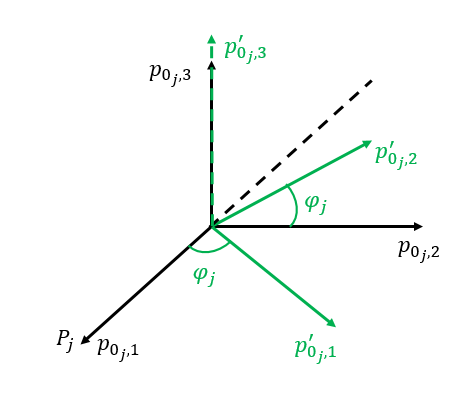
\includegraphics[width=8cm]{Figures/rotationaxes.PNG}
	\caption{Rotation Axes}
	\label{fig:Axes_Figure}
\end{figure}

\begin{equation}
	\bm{\hat{p}}_{0_j,3}=
	\leftidx{^{\mathcal{P}_{0,j}}}
	{\begin{bmatrix}
			0 \\ 0 \\ 1
	\end{bmatrix}}
\end{equation}


\begin{multline}
	m_j l_j^2\bigg[\ddot{\varphi}_j\cos^2(\vartheta_j)-2\dot{\varphi}_j\dot{\vartheta}\cos(\vartheta_j)\sin(\vartheta_j)\bigg] + m_j \bm{\hat{p}}_{0_j,3}^T \bm{l_j}\times \bigg[\bm{\dot{\omega}}_{B/N}\times \bm{l_j} + 2\bm\omega_{\cal B/N}\times \bm{l_j'}+\bm\omega_{\cal B/N}\times(\bm\omega_{\cal B/N}\times \bm{l_j})\bigg]\\
	=\bm{\hat{p}}_{0_j,3}^T \bm{L}_{T,j}+m_{j} \bm{\hat{p}}_{0_j,3}^T \bm{\ddot{r}}_{T/N}\times \bm{l_j}
	\label{eq:FSE4}
\end{multline}

\begin{equation}
	\bm{\hat{p}'}_{0_j,2}=
	\leftidx{^{\mathcal{P}_{0,j}}}
	{\begin{bmatrix}
			-\sin(\varphi) \\ \cos(\varphi) \\ 0
	\end{bmatrix}}
\end{equation}

\begin{multline}
	m_j l_j^2\bigg[\ddot{\vartheta}_j+\dot{\varphi}_j^2\cos(\vartheta_j)\sin(\vartheta_j)\bigg] + m_j \bm{\hat{p}}_{0_j,2}^{'T} \bm{l_j}\times \bigg[\bm{\dot{\omega}}_{B/N}\times \bm{l_j} + 2\bm\omega_{\cal B/N}\times \bm{l_j'}+\bm\omega_{\cal B/N}\times(\bm\omega_{\cal B/N}\times \bm{l_j})\bigg]\\
	=\bm{\hat{p}}_{0_j,2}^{'T} \bm{L}_{T,j}+m_{j} \bm{\hat{p}}_{0_j,2}^{'T} \bm{\ddot{r}}_{T/N}\times \bm{l_j}
	\label{eq:FSE5}
\end{multline}
Remembering that $\bm{r}_{T/N} = \bm{r}_{B/N} + \bm{d}$, and that $\bm{d}$ is constant in the body frame, we can use once again the transport theorem to write:

\begin{equation}
	\bm{\ddot{d}}=\bm{\dot{\omega}}_{B/N}\times \bm{d}+\bm\omega_{\cal B/N}\times(\bm\omega_{\cal B/N}\times \bm{d})
\end{equation}
\begin{equation}
	\bm{\ddot{r}}_{T/N} = \bm{\ddot{r}}_{B/N} + \bm{\dot{\omega}}_{B/N}\times \bm{d}+\bm\omega_{\cal B/N}\times(\bm\omega_{\cal B/N}\times \bm{d})
\end{equation}
Rearranging the terms as done in the previous sections
\begin{multline}
	m_j l_j^2\ddot{\varphi}_j\cos^2(\vartheta_j) -m_{j} \bm{\hat{p}}_{0_j,3}^T [\bm{\tilde{l}_j}]([\bm{\tilde{l}_j}]+ [\bm{\tilde{d}}]) \bm{\dot{\omega}}_{B/N} +m_{j} \bm{\hat{p}}_{0_j,3}^{T} [\bm{\tilde{l}_j}] \bm{\ddot{r}}_{B/N} =-m_{j} \bm{\hat{p}}_{0_j,3}^{T} [\bm{\tilde{l}_j}][\bm{\tilde{\omega}}_{\cal B/N}][\bm{\tilde{\omega}}_{\cal B/N}] \bm{d}\\+\bm{\hat{p}}_{0_j,3}^T \bm{L}_{T,j}+2m_j l_j^2\dot{\varphi}_j\dot{\vartheta}\cos(\vartheta_j)\sin(\vartheta_j)- m_j \bm{\hat{p}}_{0_j,3}^T [\bm{\tilde{l}_j}]\bigg[2[\bm{\tilde{\omega}}_{\cal B/N}] \bm{l_j'}+[\bm{\tilde{\omega}}_{\cal B/N}][\bm{\tilde{\omega}}_{\cal B/N}] \bm{l_j}\bigg]
	\label{eq:FSE6}
\end{multline}

\begin{multline}
	m_j l_j^2\ddot{\vartheta}_j - m_{j}\bm{\hat{p}}_{0_j,2}^{'T} [\bm{\tilde{l}_j}]( [\bm{\tilde{l}_j}] + [\bm{\tilde{d}}])\bm{\dot{\omega}}_{B/N}
	+m_{j} \bm{\hat{p}}_{0_j,2}^{'T} [\bm{\tilde{l}_j}] \bm{\ddot{r}}_{B/N}
	=-m_{j} \bm{\hat{p}}_{0_j,2}^{'T}[\bm{\tilde{l}_j}][\bm{\tilde{\omega}}_{\cal B/N}][\bm{\tilde{\omega}}_{\cal B/N}] \bm{d}\\+\bm{\hat{p}}_{0_j,2}^{'T} \bm{L}_{T,j}-m_j l_j^2\dot{\varphi}_j^2\cos(\vartheta_j)\sin(\vartheta_j)- m_j \bm{\hat{p}}_{0_j,2}^{'T} [\bm{\tilde{l}_j}]\bigg[2[\bm{\tilde{\omega}}_{\cal B/N}] \bm{l_j'}+[\bm{\tilde{\omega}}_{\cal B/N}][\bm{\tilde{\omega}}_{\cal B/N}] \bm{l_j}\bigg]
	\label{eq:FSE7}
\end{multline}

Eqs. \eqref{eq:FSE6} and \eqref{eq:FSE7} are the Fuel Slosh Particle equations.


\subsection{Back-substitution Method}

The equations presented in the previous sections result in $2N_P + 6$ coupled differential equations. Therefore, if the EOMs were placed into state space form, a system mass matrix of size $2N_P + 6$ would need to be inverted to numerically integrate the EOMs. This can result in a computationally expensive simulation. The computation effort to numerically invert an $N\times N$ matrix scales with $N^{3}$. In the following section, the EOMs are manipulated using a back-substitution method to increase the computational efficiency. 

This manipulation involves inverting twice a ($3\times 3$) matrix, the $A^{-1}$ and $(D-CA^{-1}B)^{-1}$ matrices as it is shown in eqs. \eqref{eq:finalsystemomega}  and \eqref{eq:finalsystemr}. Then the system is completely solved back substituting for fuel slosh and translational motions. The derivation of the back-substitution method can be seen in the following sections. 
\\

\subsubsection{Fuel Slosh Motion}
Starting from eq. \eqref{eq:FSE6}
\begin{multline}
	\ddot{\varphi}_j  =\frac{1}{m_j l_j^2 \cos^2(\vartheta_j)}\Big\{m_{j}\bm{\hat{p}}_{0_j,3}^T [\bm{\tilde{l}_j}]( [\bm{\tilde{l}_j}]+[\bm{\tilde{d}}]) \bm{\dot{\omega}}_{B/N} -m_{j} \bm{\hat{p}}_{0_j,3}^{T} [\bm{\tilde{l}_j}] \bm{\ddot{r}}_{B/N} -m_{j} \bm{\hat{p}}_{0_j,3}^{T} [\bm{\tilde{l}_j}][\bm{\tilde{\omega}}_{\cal B/N}][\bm{\tilde{\omega}}_{\cal B/N}] \bm{d}\\+\bm{\hat{p}}_{0_j,3}^T \bm{L}_{T,j}+2m_j l_j^2\dot{\varphi}_j\dot{\vartheta}\cos(\vartheta_j)\sin(\vartheta_j)- m_j \bm{\hat{p}}_{0_j,3}^T [\bm{\tilde{l}_j}]\bigg[2[\bm{\tilde{\omega}}_{\cal B/N}] \bm{l_j'}+[\bm{\tilde{\omega}}_{\cal B/N}][\bm{\tilde{\omega}}_{\cal B/N}] \bm{l_j}\bigg]\Big\}
	\label{eq:BSM1}
\end{multline}

\begin{equation}
	\ddot{\varphi}_j  =\frac{1}{m_j l_j^2 \cos^2(\vartheta_j)}\Big(m_{j}\bm{\hat{p}}_{0_j,3}^T [\bm{\tilde{l}_j}](  [\bm{\tilde{l}_j}]+ [\bm{\tilde{d}}]) \bm{\dot{\omega}}_{B/N} -m_{j} \bm{\hat{p}}_{0_j,3}^{T} [\bm{\tilde{l}_j}] \bm{\ddot{r}}_{B/N}+a_{\varphi_j} \Big)
	\label{eq:BSM2}
\end{equation}	
Writing it this way instead
\begin{equation}
	\ddot{\varphi}_j  = \bm a_{\varphi_j}^T \ddot{\bm{r}}_{B/N} + \bm b_{\varphi_j}^T \dot{\bm\omega}_{\cal B/N} +c_{\varphi_j}
	\label{eq:BSM3}
\end{equation}
Where 

\begin{equation}
	\bm a_{\varphi_j}^{T} = -\frac{\bm{\hat{p}}_{0_j,3}^{T} [\bm{\tilde{l}_j}]}{ l_j^2 \cos^2(\vartheta_j)}
	\label{eq:BSM4}
\end{equation}

\begin{equation}
	\bm b_{\varphi_j}^{T} = \frac{\bm{\hat{p}}_{0_j,3}^T [\bm{\tilde{l}_j}]( [\bm{\tilde{l}_j}]+ [\bm{\tilde{d}}])}{ l_j^2 \cos^2(\vartheta_j)}
	\label{eq:BSM5}
\end{equation}

\begin{multline}
	c_{\varphi_j} = \frac{1}{m_j l_j^2 \cos^2(\vartheta_j)}\Big\{-m_{j} \bm{\hat{p}}_{0_j,3}^{T} [\bm{\tilde{l}_j}][\bm{\tilde{\omega}}_{\cal B/N}][\bm{\tilde{\omega}}_{\cal B/N}] \bm{d}+\bm{\hat{p}}_{0_j,3}^T \bm{L}_{T,j}\\+2m_j l_j^2\dot{\varphi}_j\dot{\vartheta}\cos(\vartheta_j)\sin(\vartheta_j)- m_j \bm{\hat{p}}_{0_j,3}^T [\bm{\tilde{l}_j}]\bigg[2[\bm{\tilde{\omega}}_{\cal B/N}] \bm{l_j'}+[\bm{\tilde{\omega}}_{\cal B/N}][\bm{\tilde{\omega}}_{\cal B/N}] \bm{l_j}\bigg]\Big\}
	\label{eq:BSM6}
\end{multline}	
Doing the same for eq. \eqref{eq:FSE7}

\begin{multline}
	\ddot{\vartheta}_j 
	=\frac{1}{m_j l_j^2}\Big\{m_{j}\bm{\hat{p}}_{0_j,2}^{'T} [\bm{\tilde{l}_j}]( [\bm{\tilde{l}_j}] + [\bm{\tilde{d}}])\bm{\dot{\omega}}_{B/N}
	-m_{j} \bm{\hat{p}}_{0_j,2}^{'T} [\bm{\tilde{l}_j}] \bm{\ddot{r}}_{B/N}-m_{j} \bm{\hat{p}}_{0_j,2}^{'T}[\bm{\tilde{l}_j}][\bm{\tilde{\omega}}_{\cal B/N}][\bm{\tilde{\omega}}_{\cal B/N}] \bm{d}\\+\bm{\hat{p}}_{0_j,2}^{'T} \bm{L}_{T,j}-m_j l_j^2\dot{\varphi}_j^2\cos(\vartheta_j)\sin(\vartheta_j)- m_j \bm{\hat{p}}_{0_j,2}^{'T} [\bm{\tilde{l}_j}]\bigg[2[\bm{\tilde{\omega}}_{\cal B/N}] \bm{l_j'}+[\bm{\tilde{\omega}}_{\cal B/N}][\bm{\tilde{\omega}}_{\cal B/N}] \bm{l_j}\bigg]\Big\}
	\label{eq:BSM7}
\end{multline}

\begin{equation}
	\ddot \vartheta_j =\frac{1}{m_j l_j^2} \Big(m_{j}\bm{\hat{p}}_{0_j,2}^{'T} [\bm{\tilde{l}_j}]([\bm{\tilde{l}_j}] + [\bm{\tilde{d}}])\bm{\dot{\omega}}_{B/N}
	-m_{j} \bm{\hat{p}}_{0_j,2}^{'T} [\bm{\tilde{l}_j}] \bm{\ddot{r}}_{B/N} + a_{\vartheta_j} \Big)
	\label{eq:BSM8}
\end{equation}
Writing this a different way

\begin{equation}
	\ddot \vartheta_j = \bm a_{\vartheta_j}^T \ddot{\bm r}_{B/N} + \bm b_{\vartheta_j}^T \dot{\bm\omega}_{\cal B/N} + c_{\vartheta_j}
	\label{eq:BSM9}
\end{equation}
Where

\begin{equation}
	\bm a_{\vartheta_j}^{T} = - \frac{ \bm{\hat{p}}_{0_j,2}^{'T} [\bm{\tilde{l}_j}]}{ l_j^2}
	\label{eq:BSM10}
\end{equation}

\begin{equation}
	\bm b_{\vartheta_j}^{T} = \frac{\bm{\hat{p}}_{0_j,2}^{'T} [\bm{\tilde{l}_j}]( [\bm{\tilde{l}_j}] + [\bm{\tilde{d}}])}{ l_j^2}
	\label{eq:BSM11}
\end{equation}

\begin{multline}
	c_{\vartheta_j} = \frac{1}{m_j l_j^2}\Big\{-m_{j} \bm{\hat{p}}_{0_j,2}^{'T}[\bm{\tilde{l}_j}][\bm{\tilde{\omega}}_{\cal B/N}][\bm{\tilde{\omega}}_{\cal B/N}] \bm{d}+\bm{\hat{p}}_{0_j,2}^{'T} \bm{L}_{T,j}-m_j l_j^2\dot{\varphi}_j^2\cos(\vartheta_j)\sin(\vartheta_j)\\- m_j \bm{\hat{p}}_{0_j,2}^{'T} [\bm{\tilde{l}_j}]\bigg[2[\bm{\tilde{\omega}}_{\cal B/N}] \bm{l_j'}+[\bm{\tilde{\omega}}_{\cal B/N}][\bm{\tilde{\omega}}_{\cal B/N}] \bm{l_j}\bigg] \Big\}
	\label{eq:BSM12}
\end{multline}

\subsubsection{Translation}

Plugging these definitions into the translation equation

\begin{multline}
	\ddot{\bm r}_{B/N}-[\tilde{\bm{c}}] \dot{\bm\omega}_{\cal B/N}-\frac{1}{m_{\text{sc}}}\sum_{j=1}^{N_{P}}m_j l_j \bigg[
	\Big(\sin(\varphi_j)\cos(\vartheta_j)\bm{\hat{p}}_{0_j,1}-\cos(\varphi_j)\cos(\vartheta_j)\bm{\hat{p}}_{0_j,2}\Big)\ddot{\varphi}_j \\+\Big(\cos(\varphi_j)\sin(\vartheta_j)\bm{\hat{p}}_{0_j,1}+\sin(\varphi_j)\sin(\vartheta_j)\bm{\hat{p}}_{0_j,2}+\cos(\vartheta_j)\bm{\hat{p}}_{0_j,3}\Big)\ddot{\vartheta}_j
	\bigg]= \ddot{\bm r}_{C/N} 	- 2[\tilde{\bm\omega}_{\cal B/N}] \bm c'
	\\-[\tilde{\bm\omega}_{\cal B/N}][\tilde{\bm\omega}_{\cal B/N}]\bm{c}
	-\frac{1}{m_{\text{sc}}}\sum_{j=1}^{N_{P}}m_j l_j \bigg[
	\Big(-\cos(\varphi_j)\cos(\vartheta_j)\bm{\hat{p}}_{0_j,1}-\sin(\varphi_j)\cos(\vartheta_j)\bm{\hat{p}}_{0_j,2}\Big)\dot{\varphi}_j^2
	\\+\Big(-\cos(\varphi_j)\cos(\vartheta_j)\bm{\hat{p}}_{0_j,1}-\sin(\varphi_j)\cos(\vartheta_j)\bm{\hat{p}}_{0_j,2}+\sin(\vartheta_j)\bm{\hat{p}}_{0_j,3} \Big)\dot{\vartheta}_j^2 \\+
	\Big(2\sin(\varphi_j)\sin(\vartheta_j)\bm{\hat{p}}_{0_j,1} -2\cos(\varphi_j)\sin(\vartheta_j)\bm{\hat{p}}_{0_j,2}\Big)\dot{\varphi}_j\dot{\vartheta}_j
	\bigg]
	\label{eq:Rbddot4_bis}
\end{multline}
Results in

\begin{multline}
	\ddot{\bm r}_{B/N}-[\tilde{\bm{c}}] \dot{\bm\omega}_{\cal B/N}-\frac{1}{m_{\text{sc}}}\sum_{j=1}^{N_{P}}m_j l_j \bigg[
	\Big(\sin(\varphi_j)\cos(\vartheta_j)\bm{\hat{p}}_{0_j,1}-\cos(\varphi_j)\cos(\vartheta_j)\bm{\hat{p}}_{0_j,2}\Big)(\bm a_{\varphi_j}^T \ddot{\bm{r}}_{B/N} + \bm b_{\varphi_j}^T \dot{\bm\omega}_{\cal B/N} +c_{\varphi_j}) \\ +\Big(\cos(\varphi_j)\sin(\vartheta_j)\bm{\hat{p}}_{0_j,1}+\sin(\varphi_j)\sin(\vartheta_j)\bm{\hat{p}}_{0_j,2}+\cos(\vartheta_j)\bm{\hat{p}}_{0_j,3}\Big)(\bm a_{\vartheta_j}^T \ddot{\bm r}_{B/N} + \bm b_{\vartheta_j}^T \dot{\bm\omega}_{\cal B/N} + c_{\vartheta_j})
	\bigg]
	\\= \ddot{\bm r}_{C/N} 	- 2[\tilde{\bm\omega}_{\cal B/N}] \bm c'
	-[\tilde{\bm\omega}_{\cal B/N}][\tilde{\bm\omega}_{\cal B/N}]\bm{c}
	-\frac{1}{m_{\text{sc}}}\sum_{j=1}^{N_{P}}m_j l_j \bigg[
	\Big(-\cos(\varphi_j)\cos(\vartheta_j)\bm{\hat{p}}_{0_j,1}-\sin(\varphi_j)\cos(\vartheta_j)\bm{\hat{p}}_{0_j,2}\Big)\dot{\varphi}_j^2\\
	+\Big(-\cos(\varphi_j)\cos(\vartheta_j)\bm{\hat{p}}_{0_j,1}-\sin(\varphi_j)\cos(\vartheta_j)\bm{\hat{p}}_{0_j,2}+\sin(\vartheta_j)\bm{\hat{p}}_{0_j,3} \Big)\dot{\vartheta}_j^2\\ +
	\Big(2\sin(\varphi_j)\sin(\vartheta_j)\bm{\hat{p}}_{0_j,1} -2\cos(\varphi_j)\sin(\vartheta_j)\bm{\hat{p}}_{0_j,2}\Big)\dot{\varphi}_j\dot{\vartheta}_j
	\bigg]
	\label{eq:Rbddot5}
\end{multline}
Simplifying

\begin{multline}
	\Big\{[I_{3\times3}] -\frac{1}{m_{\text{sc}}}\sum_{j=1}^{N_{P}}m_j l_j \bigg[
	\Big(\sin(\varphi_j)\cos(\vartheta_j)\bm{\hat{p}}_{0_j,1}-\cos(\varphi_j)\cos(\vartheta_j)\bm{\hat{p}}_{0_j,2}\Big)\bm a_{\varphi_j}^T +\Big(\cos(\varphi_j)\sin(\vartheta_j)\bm{\hat{p}}_{0_j,1}\\+\sin(\varphi_j)\sin(\vartheta_j)\bm{\hat{p}}_{0_j,2}+\cos(\vartheta_j)\bm{\hat{p}}_{0_j,3}\Big)\bm a_{\vartheta_j}^T \bigg]\Big\}\ddot{\bm r}_{B/N}
	+\Big\{-[\tilde{\bm{c}}] -\frac{1}{m_{\text{sc}}}\sum_{j=1}^{N_{P}}m_j l_j \bigg[
	\Big(\sin(\varphi_j)\cos(\vartheta_j)\bm{\hat{p}}_{0_j,1}\\-\cos(\varphi_j)\cos(\vartheta_j)\bm{\hat{p}}_{0_j,2}\Big)\bm b_{\varphi_j}^T +\Big(\cos(\varphi_j)\sin(\vartheta_j)\bm{\hat{p}}_{0_j,1}+\sin(\varphi_j)\sin(\vartheta_j)\bm{\hat{p}}_{0_j,2}+\cos(\vartheta_j)\bm{\hat{p}}_{0_j,3}\Big)\bm b_{\vartheta_j}^T \bigg] \Big\}\dot{\bm\omega}_{\cal B/N}
	\\= \ddot{\bm r}_{C/N} 	- 2[\tilde{\bm\omega}_{\cal B/N}] \bm c'
	-[\tilde{\bm\omega}_{\cal B/N}][\tilde{\bm\omega}_{\cal B/N}]\bm{c}
	-\frac{1}{m_{\text{sc}}}\sum_{j=1}^{N_{P}}m_j l_j \bigg[ 
	\Big(-\cos(\varphi_j)\cos(\vartheta_j)\bm{\hat{p}}_{0_j,1}\\-\sin(\varphi_j)\cos(\vartheta_j)\bm{\hat{p}}_{0_j,2}\Big)\dot{\varphi}_j^2
	+\Big(-\cos(\varphi_j)\cos(\vartheta_j)\bm{\hat{p}}_{0_j,1}-\sin(\varphi_j)\cos(\vartheta_j)\bm{\hat{p}}_{0_j,2}+\sin(\vartheta_j)\bm{\hat{p}}_{0_j,3} \Big)\dot{\vartheta}_j^2 \\+
	\Big(2\sin(\varphi_j)\sin(\vartheta_j)\bm{\hat{p}}_{0_j,1} -2\cos(\varphi_j)\sin(\vartheta_j)\bm{\hat{p}}_{0_j,2}\Big)\dot{\varphi}_j\dot{\vartheta}_j
	-\Big(\sin(\varphi_j)\cos(\vartheta_j)\bm{\hat{p}}_{0_j,1}\\-\cos(\varphi_j)\cos(\vartheta_j)\bm{\hat{p}}_{0_j,2}\Big)c_{\varphi_j} - \Big(\cos(\varphi_j)\sin(\vartheta_j)\bm{\hat{p}}_{0_j,1}+\sin(\varphi_j)\sin(\vartheta_j)\bm{\hat{p}}_{0_j,2}+\cos(\vartheta_j)\bm{\hat{p}}_{0_j,3}\Big) c_{\vartheta_j} 
	\bigg]
	\label{eq:Rbddot6}
\end{multline}
Multiply both sides by $m_{\text{sc}}$.

\begin{multline}
	\Big\{m_{\text{sc}}[I_{3\times3}] -\sum_{j=1}^{N_{P}}m_j l_j \bigg[
	\Big(\sin(\varphi_j)\cos(\vartheta_j)\bm{\hat{p}}_{0_j,1}-\cos(\varphi_j)\cos(\vartheta_j)\bm{\hat{p}}_{0_j,2}\Big)\bm a_{\varphi_j}^T +\Big(\cos(\varphi_j)\sin(\vartheta_j)\bm{\hat{p}}_{0_j,1}\\+\sin(\varphi_j)\sin(\vartheta_j)\bm{\hat{p}}_{0_j,2}+\cos(\vartheta_j)\bm{\hat{p}}_{0_j,3}\Big)\bm a_{\vartheta_j}^T \bigg]\Big\}\ddot{\bm r}_{B/N}
	+\Big\{-m_{\text{sc}}[\tilde{\bm{c}}] -\sum_{j=1}^{N_{P}}m_j l_j \bigg[
	\Big(\sin(\varphi_j)\cos(\vartheta_j)\bm{\hat{p}}_{0_j,1}\\-\cos(\varphi_j)\cos(\vartheta_j)\bm{\hat{p}}_{0_j,2}\Big)\bm b_{\varphi_j}^T +\Big(\cos(\varphi_j)\sin(\vartheta_j)\bm{\hat{p}}_{0_j,1}+\sin(\varphi_j)\sin(\vartheta_j)\bm{\hat{p}}_{0_j,2}+\cos(\vartheta_j)\bm{\hat{p}}_{0_j,3}\Big)\bm b_{\vartheta_j}^T \bigg] \Big\}\dot{\bm\omega}_{\cal B/N}
	\\= m_{\text{sc}}\ddot{\bm r}_{C/N} - 2m_{\text{sc}}[\tilde{\bm\omega}_{\cal B/N}] \bm c'
	-m_{\text{sc}}[\tilde{\bm\omega}_{\cal B/N}][\tilde{\bm\omega}_{\cal B/N}]\bm{c}
	-\sum_{j=1}^{N_{P}}m_j l_j \bigg[ 
	\Big(-\cos(\varphi_j)\cos(\vartheta_j)\bm{\hat{p}}_{0_j,1}\\-\sin(\varphi_j)\cos(\vartheta_j)\bm{\hat{p}}_{0_j,2}\Big)\dot{\varphi}_j^2
	+\Big(-\cos(\varphi_j)\cos(\vartheta_j)\bm{\hat{p}}_{0_j,1}-\sin(\varphi_j)\cos(\vartheta_j)\bm{\hat{p}}_{0_j,2}+\sin(\vartheta_j)\bm{\hat{p}}_{0_j,3} \Big)\dot{\vartheta}_j^2 \\+
	\Big(2\sin(\varphi_j)\sin(\vartheta_j)\bm{\hat{p}}_{0_j,1} -2\cos(\varphi_j)\sin(\vartheta_j)\bm{\hat{p}}_{0_j,2}\Big)\dot{\varphi}_j\dot{\vartheta}_j
	-\Big(\sin(\varphi_j)\cos(\vartheta_j)\bm{\hat{p}}_{0_j,1}\\-\cos(\varphi_j)\cos(\vartheta_j)\bm{\hat{p}}_{0_j,2}\Big)c_{\varphi_j} - \Big(\cos(\varphi_j)\sin(\vartheta_j)\bm{\hat{p}}_{0_j,1}+\sin(\varphi_j)\sin(\vartheta_j)\bm{\hat{p}}_{0_j,2}+\cos(\vartheta_j)\bm{\hat{p}}_{0_j,3}\Big) c_{\vartheta_j} 
	\bigg]
	\label{eq:Rbddot7}
\end{multline}

\subsubsection{Rotation}

Same thing for rotation: 

\begin{multline}
	m_{\text{sc}}[\tilde{\bm{c}}]\ddot{\bm r}_{B/N}+[I_{\text{sc},B}] \dot{\bm\omega}_{\cal B/N}  - \sum\limits_{j=1}^{N_P}m_j l_j [\tilde{\bm{r}}_{P_{c,j}/B}] \bigg[
	\Big(\sin(\varphi_j)\cos(\vartheta_j)\bm{\hat{p}}_{0_j,1}\\-\cos(\varphi_j)\cos(\vartheta_j)\bm{\hat{p}}_{0_j,2}\Big)(\bm a_{\varphi_j}^T \ddot{\bm{r}}_{B/N} + \bm b_{\varphi_j}^T \dot{\bm\omega}_{\cal B/N}+c_{\varphi_j}) 
	+\Big(\cos(\varphi_j)\sin(\vartheta_j)\bm{\hat{p}}_{0_j,1}+\sin(\varphi_j)\sin(\vartheta_j)\bm{\hat{p}}_{0_j,2}\\+\cos(\vartheta_j)\bm{\hat{p}}_{0_j,3} \Big)(\bm a_{\vartheta_j}^T \ddot{\bm r}_{B/N} + \bm b_{\vartheta_j}^T \dot{\bm\omega}_{\cal B/N} + c_{\vartheta_j})
	\bigg] = \\
	\bm{L}_B-[\bm{\tilde{\omega}}_{\cal B/N}] [I_{\text{sc},B}] \bm\omega_{\cal B/N}
	- [I'_{\text{sc},B}] \bm\omega_{\cal B/N}- \sum\limits_{j=1}^{N_P} m_j \Big\{[\tilde{\bm\omega}_{\cal B/N}] [\tilde{\bm{r}}_{P_{c,j}/B}] \bm{r}'_{P_{c,j}/B}\\
	+l_j[\tilde{\bm{r}}_{P_{c,j}/B}]\bigg[
	\Big(-\cos(\varphi_j)\cos(\vartheta_j)\bm{\hat{p}}_{0_j,1}-\sin(\varphi_j)\cos(\vartheta_j)\bm{\hat{p}}_{0_j,2}\Big)\dot{\varphi}_j^2
	+\Big(-\cos(\varphi_j)\cos(\vartheta_j)\bm{\hat{p}}_{0_j,1}\\-\sin(\varphi_j)\cos(\vartheta_j)\bm{\hat{p}}_{0_j,2}+\sin(\vartheta_j)\bm{\hat{p}}_{0_j,3} \Big)\dot{\vartheta}_j^2 +
	\Big(2\sin(\varphi_j)\sin(\vartheta_j)\bm{\hat{p}}_{0_j,1} -2\cos(\varphi_j)\sin(\vartheta_j)\bm{\hat{p}}_{0_j,2}\Big)\dot{\varphi}_j\dot{\vartheta}_j
	\bigg]\Big\}
	\label{eq:Final6_1}
\end{multline}
Next

\begin{multline}
	\Big\{m_{\text{sc}}[\tilde{\bm{c}}] - \sum\limits_{j=1}^{N_P}m_j l_j [\tilde{\bm{r}}_{P_{c,j}/B}] \bigg[
	\Big(\sin(\varphi_j)\cos(\vartheta_j)\bm{\hat{p}}_{0_j,1}-\cos(\varphi_j)\cos(\vartheta_j)\bm{\hat{p}}_{0_j,2}\Big)\bm a_{\varphi_j}^T
	+\Big(\cos(\varphi_j)\sin(\vartheta_j)\bm{\hat{p}}_{0_j,1}\\+\sin(\varphi_j)\sin(\vartheta_j)\bm{\hat{p}}_{0_j,2}+\cos(\vartheta_j)\bm{\hat{p}}_{0_j,3} \Big)\bm a_{\vartheta_j}^T
	\bigg]
	\Big\}\ddot{\bm r}_{B/N}
	+\Big\{[I_{\text{sc},B}] - \sum\limits_{j=1}^{N_P}m_j l_j [\tilde{\bm{r}}_{P_{c,j}/B}] \bigg[
	\Big(\sin(\varphi_j)\cos(\vartheta_j)\bm{\hat{p}}_{0_j,1}\\-\cos(\varphi_j)\cos(\vartheta_j)\bm{\hat{p}}_{0_j,2}\Big)\bm b_{\varphi_j}^T
	+\Big(\cos(\varphi_j)\sin(\vartheta_j)\bm{\hat{p}}_{0_j,1}
	+\sin(\varphi_j)\sin(\vartheta_j)\bm{\hat{p}}_{0_j,2}+\cos(\vartheta_j)\bm{\hat{p}}_{0_j,3} \Big)\bm b_{\vartheta_j}^T
	\bigg]
	\Big\}\dot{\bm\omega}_{\cal B/N}
	\\= 
	\bm{L}_B-[\bm{\tilde{\omega}}_{\cal B/N}] [I_{\text{sc},B}] \bm\omega_{\cal B/N}
	- [I'_{\text{sc},B}] \bm\omega_{\cal B/N}- \sum\limits_{j=1}^{N_P} m_j \Big\{[\tilde{\bm\omega}_{\cal B/N}] [\tilde{\bm{r}}_{P_{c,j}/B}] \bm{r}'_{P_{c,j}/B}
	\\+l_j[\tilde{\bm{r}}_{P_{c,j}/B}]\bigg[
	\Big(-\cos(\varphi_j)\cos(\vartheta_j)\bm{\hat{p}}_{0_j,1}-\sin(\varphi_j)\cos(\vartheta_j)\bm{\hat{p}}_{0_j,2}\Big)\dot{\varphi}_j^2
	+\Big(-\cos(\varphi_j)\cos(\vartheta_j)\bm{\hat{p}}_{0_j,1}\\-\sin(\varphi_j)\cos(\vartheta_j)\bm{\hat{p}}_{0_j,2}+\sin(\vartheta_j)\bm{\hat{p}}_{0_j,3} \Big)\dot{\vartheta}_j^2 +
	\Big(2\sin(\varphi_j)\sin(\vartheta_j)\bm{\hat{p}}_{0_j,1} \\-2\cos(\varphi_j)\sin(\vartheta_j)\bm{\hat{p}}_{0_j,2}\Big)\dot{\varphi}_j\dot{\vartheta}_j
	- \Big(\sin(\varphi_j)\cos(\vartheta_j)\bm{\hat{p}}_{0_j,1} -\cos(\varphi_j)\cos(\vartheta_j)\bm{\hat{p}}_{0_j,2}\Big)c_{\varphi_j} \\-   \Big(\cos(\varphi_j)\sin(\vartheta_j)\bm{\hat{p}}_{0_j,1}+\sin(\varphi_j)\sin(\vartheta_j)\bm{\hat{p}}_{0_j,2}+\cos(\vartheta_j)\bm{\hat{p}}_{0_j,3}\Big) c_{\vartheta_j}
	\bigg]\Big\}
	\label{eq:Final7}
\end{multline}

\subsubsection{Remaining Back-substitution Steps}

The following definitions can be defined:

\begin{multline}
	[A] = \Big\{m_{\text{sc}}[I_{3\times3}] -\sum_{j=1}^{N_{P}}m_j l_j \bigg[
	\Big(\sin(\varphi_j)\cos(\vartheta_j)\bm{\hat{p}}_{0_j,1}-\cos(\varphi_j)\cos(\vartheta_j)\bm{\hat{p}}_{0_j,2}\Big)\bm a_{\varphi_j}^T \\ +\Big(\cos(\varphi_j)\sin(\vartheta_j)\bm{\hat{p}}_{0_j,1}+\sin(\varphi_j)\sin(\vartheta_j)\bm{\hat{p}}_{0_j,2}+\cos(\vartheta_j)\bm{\hat{p}}_{0_j,3}\Big)\bm a_{\vartheta_j}^T \bigg]\Big\}
\end{multline}

\begin{multline}
	[B] = 	\Big\{-m_{\text{sc}}[\tilde{\bm{c}}] -\sum_{j=1}^{N_{P}}m_j l_j \bigg[
	\Big(\sin(\varphi_j)\cos(\vartheta_j)\bm{\hat{p}}_{0_j,1}-\cos(\varphi_j)\cos(\vartheta_j)\bm{\hat{p}}_{0_j,2}\Big)\bm b_{\varphi_j}^T\\ +\Big(\cos(\varphi_j)\sin(\vartheta_j)\bm{\hat{p}}_{0_j,1}+\sin(\varphi_j)\sin(\vartheta_j)\bm{\hat{p}}_{0_j,2}+\cos(\vartheta_j)\bm{\hat{p}}_{0_j,3}\Big)\bm b_{\vartheta_j}^T \bigg] \Big\}
\end{multline}

\begin{multline}
	[C] = \Big\{m_{\text{sc}}[\tilde{\bm{c}}] - \sum\limits_{j=1}^{N_P}m_j l_j [\tilde{\bm{r}}_{P_{c,j}/B}] \bigg[
	\Big(\sin(\varphi_j)\cos(\vartheta_j)\bm{\hat{p}}_{0_j,1}-\cos(\varphi_j)\cos(\vartheta_j)\bm{\hat{p}}_{0_j,2}\Big)\bm a_{\varphi_j}^T \\
	+\Big(\cos(\varphi_j)\sin(\vartheta_j)\bm{\hat{p}}_{0_j,1}+\sin(\varphi_j)\sin(\vartheta_j)\bm{\hat{p}}_{0_j,2}+\cos(\vartheta_j)\bm{\hat{p}}_{0_j,3} \Big)\bm a_{\vartheta_j}^T
	\bigg]
	\Big\}
\end{multline}

\begin{multline}
	[D] = \Big\{[I_{\text{sc},B}] - \sum\limits_{j=1}^{N_P}m_j l_j [\tilde{\bm{r}}_{P_{c,j}/B}] \bigg[
	\Big(\sin(\varphi_j)\cos(\vartheta_j)\bm{\hat{p}}_{0_j,1}-\cos(\varphi_j)\cos(\vartheta_j)\bm{\hat{p}}_{0_j,2}\Big)\bm b_{\varphi_j}^T \\
	+\Big(\cos(\varphi_j)\sin(\vartheta_j)\bm{\hat{p}}_{0_j,1}
	+\sin(\varphi_j)\sin(\vartheta_j)\bm{\hat{p}}_{0_j,2}+\cos(\vartheta_j)\bm{\hat{p}}_{0_j,3} \Big)\bm b_{\vartheta_j}^T
	\bigg]
	\Big\}
\end{multline}

\begin{multline}
	\bm v_{\text{trans}} = m_{\text{sc}}\ddot{\bm r}_{C/N} - 2m_{\text{sc}}[\tilde{\bm\omega}_{\cal B/N}] \bm c'
	-m_{\text{sc}}[\tilde{\bm\omega}_{\cal B/N}][\tilde{\bm\omega}_{\cal B/N}]\bm{c}
	\\-\sum_{j=1}^{N_{P}}m_j l_j \bigg[ 
	\Big(-\cos(\varphi_j)\cos(\vartheta_j)\bm{\hat{p}}_{0_j,1}-\sin(\varphi_j)\cos(\vartheta_j)\bm{\hat{p}}_{0_j,2}\Big)\dot{\varphi}_j^2
	+\Big(-\cos(\varphi_j)\cos(\vartheta_j)\bm{\hat{p}}_{0_j,1}\\-\sin(\varphi_j)\cos(\vartheta_j)\bm{\hat{p}}_{0_j,2}+\sin(\vartheta_j)\bm{\hat{p}}_{0_j,3} \Big)\dot{\vartheta}_j^2 +
	\Big(2\sin(\varphi_j)\sin(\vartheta_j)\bm{\hat{p}}_{0_j,1}\\ -2\cos(\varphi_j)\sin(\vartheta_j)\bm{\hat{p}}_{0_j,2}\Big)\dot{\varphi}_j\dot{\vartheta}_j
	-\Big(\sin(\varphi_j)\cos(\vartheta_j)\bm{\hat{p}}_{0_j,1}-\cos(\varphi_j)\cos(\vartheta_j)\bm{\hat{p}}_{0_j,2}\Big)c_{\varphi_j}\\ - \Big(\cos(\varphi_j)\sin(\vartheta_j)\bm{\hat{p}}_{0_j,1}+\sin(\varphi_j)\sin(\vartheta_j)\bm{\hat{p}}_{0_j,2}+\cos(\vartheta_j)\bm{\hat{p}}_{0_j,3}\Big) c_{\vartheta_j} 
	\bigg]
\end{multline}

\begin{multline}
	\bm v_{\text{rot}} = 	\bm{L}_B-[\bm{\tilde{\omega}}_{\cal B/N}] [I_{\text{sc},B}] \bm\omega_{\cal B/N}
	- [I'_{\text{sc},B}] \bm\omega_{\cal B/N}\\- \sum\limits_{j=1}^{N_P} m_j \Big\{[\tilde{\bm\omega}_{\cal B/N}] [\tilde{\bm{r}}_{P_{c,j}/B}] \bm{r}'_{P_{c,j}/B}
	+l_j[\tilde{\bm{r}}_{P_{c,j}/B}]\bigg[
	\Big(-\cos(\varphi_j)\cos(\vartheta_j)\bm{\hat{p}}_{0_j,1} -\sin(\varphi_j)\cos(\vartheta_j)\bm{\hat{p}}_{0_j,2}\Big)\dot{\varphi}_j^2
	\\+\Big(-\cos(\varphi_j)\cos(\vartheta_j)\bm{\hat{p}}_{0_j,1}-\sin(\varphi_j)\cos(\vartheta_j)\bm{\hat{p}}_{0_j,2}+\sin(\vartheta_j)\bm{\hat{p}}_{0_j,3} \Big)\dot{\vartheta}_j^2 +
	\Big(2\sin(\varphi_j)\sin(\vartheta_j)\bm{\hat{p}}_{0_j,1}\\ -2\cos(\varphi_j)\sin(\vartheta_j)\bm{\hat{p}}_{0_j,2}\Big)\dot{\varphi}_j\dot{\vartheta}_j
	-\Big(\sin(\varphi_j)\cos(\vartheta_j)\bm{\hat{p}}_{0_j,1} -\cos(\varphi_j)\cos(\vartheta_j)\bm{\hat{p}}_{0_j,2}\Big)c_{\varphi_j} \\-   \Big(\cos(\varphi_j)\sin(\vartheta_j)\bm{\hat{p}}_{0_j,1}+\sin(\varphi_j)\sin(\vartheta_j)\bm{\hat{p}}_{0_j,2}+\cos(\vartheta_j)\bm{\hat{p}}_{0_j,3}\Big) c_{\vartheta_j}
	\bigg]\Big\}
\end{multline}

Therefore the translation and rotation EOMs are written in the following form

\begin{equation}
	\begin{bmatrix}
		[A] & [B]\\
		[C] & [D]
	\end{bmatrix} \begin{bmatrix}
		\ddot{\bm r}_{B/N}\\
		\dot{\bm\omega}_{\cal B/N}
	\end{bmatrix} = \begin{bmatrix}
		\bm v_{\text{trans}}\\
		\bm v_{\text{rot}}
	\end{bmatrix}
\end{equation}

Solving the system-of-equations by

\begin{equation}
	\dot{\bm\omega}_{\cal B/N} = \Big([D] - [C]][A]^{-1}[B]\Big)^{-1}(\bm v_{\text{rot}} - [C][A]^{-1}\bm v_{\text{trans}})
	\label{eq:finalsystemomega}
\end{equation}

\begin{equation}
	\ddot{\bm r}_{B/N} = [A]^{-1} (\bm v_{\text{trans}} - [B]\dot{\bm\omega}_{\cal B/N})
	\label{eq:finalsystemr}
\end{equation}

Now the other state variables can be solved using Eqs. \eqref{eq:BSM3} and \eqref{eq:BSM9}: 

\begin{equation}
	\ddot{\varphi}_j  = \bm a_{\varphi_j}^T \ddot{\bm{r}}_{B/N} + \bm b_{\varphi_j}^T \dot{\bm\omega}_{\cal B/N} +c_{\varphi_j}
\end{equation}

\begin{equation}
	\ddot \vartheta_j = \bm a_{\vartheta_j}^T \ddot{\bm r}_{B/N} + \bm b_{\vartheta_j}^T \dot{\bm\omega}_{\cal B/N} + c_{\vartheta_j}
\end{equation}\\
\subsection{Rotational Kinetic Energy}
The total rotational kinetic energy (i.e. kinetic energy about the center of mass) of
the spacecraft is:
\begin{equation}
	T_{rot}=\frac{1}{2}\bm\omega_{\cal B/N}^T [I_{\text{hub},B_c}] \bm\omega_{\cal B/N}+\frac{1}{2}m_{\text{hub}}\bm{\dot{r}}_{B_c,C}\cdot\bm{\dot{r}}_{B_c,C}+\sum\limits_{j=1}^{N_P} \frac{1}{2} m_j \bm{\dot{r}}_{P_{c,j}/C}\cdot\bm{\dot{r}}_{P_{c,j}/C}
	\label{eq:RKE1}
\end{equation}
Expanding these terms results in
\begin{equation}
	T_{rot}=\frac{1}{2}\bm\omega_{\cal B/N}^T [I_{\text{hub},B_c}] \bm\omega_{\cal B/N}+\frac{1}{2}m_{\text{hub}}(\bm{\dot{r}}_{B_c,B}-\bm{\dot{c}})\cdot(\bm{\dot{r}}_{B_c,B}-\bm{\dot{c}})+\sum\limits_{j=1}^{N_P} \frac{1}{2} m_j (\bm{\dot{r}}_{P_{c,j}/B}-\bm{\dot{c}})\cdot(\bm{\dot{r}}_{P_{c,j}/B}-\bm{\dot{c}})
	\label{eq:RKE2}
\end{equation}
Expanding further
\begin{multline}
	T_{rot}=\frac{1}{2}\bm\omega_{\cal B/N}^T [I_{\text{hub},B_c}] \bm\omega_{\cal B/N}+\frac{1}{2}m_{\text{hub}}(\bm{\dot{r}}_{B_c,B}\cdot\bm{\dot{r}}_{B_c,B}-2\bm{\dot{r}}_{B_c,B}\cdot\bm{\dot{c}}+\bm{\dot{c}}\cdot\bm{\dot{c}})\\+\sum\limits_{j=1}^{N_P} \frac{1}{2} m_j (\bm{\dot{r}}_{P_{c,j}/B}\cdot\bm{\dot{r}}_{P_{c,j}/B}-2\bm{\dot{r}}_{P_{c,j}/B}\cdot\bm{\dot{c}}+\bm{\dot{c}}\cdot\bm{\dot{c}})
	\label{eq:RKE3}
\end{multline}
Combining like terms results in
\begin{multline}
	T_{rot}=\frac{1}{2}\bm\omega_{\cal B/N}^T [I_{\text{hub},B_c}] \bm\omega_{\cal B/N}+\frac{1}{2}m_{\text{hub}}\bm{\dot{r}}_{B_c,B}\cdot\bm{\dot{r}}_{B_c,B}+\sum\limits_{j=1}^{N_P} \frac{1}{2} m_j \bm{\dot{r}}_{P_{c,j}/B}\cdot\bm{\dot{r}}_{P_{c,j}/B}\\-\bigg[m_{\text{hub}}\bm{\dot{r}}_{B_c,B}+\sum\limits_{j=1}^{N_P} m_j \bm{\dot{r}}_{P_{c,j}/B}\bigg]\cdot\bm{\dot{c}}+\frac{1}{2}\bigg[m_{\text{hub}}+\sum\limits_{j=1}^{N_P} m_j \bigg]\bm{\dot{c}}\cdot\bm{\dot{c}}
	\label{eq:RKE3_1}
\end{multline}
Performing a final simplification yields
\begin{equation}
	T_{rot}=\frac{1}{2}\bm\omega_{\cal B/N}^T [I_{\text{hub},B_c}] \bm\omega_{\cal B/N}+\frac{1}{2}m_{\text{hub}}\bm{\dot{r}}_{B_c,B}\cdot\bm{\dot{r}}_{B_c,B}+\sum\limits_{j=1}^{N_P} \frac{1}{2} m_j \bm{\dot{r}}_{P_{c,j}/B}\cdot\bm{\dot{r}}_{P_{c,j}/B}-\frac{1}{2}m_{SC}\bm{\dot{c}}\cdot\bm{\dot{c}}
	\label{eq:RKE4}
\end{equation} \\
\subsection{Rotational Angular Momentum}
The total rotational angular momentum of the spacecraft about point C is
\begin{equation}
	\bm{H}_{rot,C}=[I_{\text{hub},B_c}] \bm\omega_{\cal B/N}+m_{\text{hub}}\bm{r}_{B_c,C}\times\bm{\dot{r}}_{B_c,C}+\sum\limits_{j=1}^{N_P}  m_j \bm{r}_{P_{c,j}/C}\times\bm{\dot{r}}_{P_{c,j}/C}
	\label{eq:RAM1}
\end{equation}
Expanding these terms yields
\begin{equation}
	\bm{H}_{rot,C}=[I_{\text{hub},B_c}] \bm\omega_{\cal B/N}+m_{\text{hub}}(\bm{r}_{B_c,B}-\bm{c})\times(\bm{\dot{r}}_{B_c,B}-\bm{\dot{c}})+\sum\limits_{j=1}^{N_P}  m_j (\bm{r}_{P_{c,j}/B}-\bm{c})\times(\bm{\dot{r}}_{P_{c,j}/B}-\bm{\dot{c}})
	\label{eq:RAM2}
\end{equation}
Distributing this result
\begin{multline}
	\bm{H}_{rot,C}=[I_{\text{hub},B_c}] \bm\omega_{\cal B/N}+m_{\text{hub}}(\bm{r}_{B_c,B}\times\bm{\dot{r}}_{B_c,B}-\bm{r}_{B_c,B}\times\bm{\dot{c}}-\bm{c}\times\bm{\dot{r}}_{B_c,B}+\bm{c}\times\bm{\dot{c}})\\+\sum\limits_{j=1}^{N_P} m_j (\bm{r}_{P_{c,j}/B}\times\bm{\dot{r}}_{P_{c,j}/B}-\bm{r}_{P_{c,j}/B}\times\bm{\dot{c}}-\bm{c}\times\bm{\dot{r}}_{P_{c,j}/B}+\bm{c}\times\bm{\dot{c}})
	\label{eq:RAM3}
\end{multline}
Simplifying this result yields the final equation
\begin{equation}
	\bm{H}_{rot,C}=[I_{\text{hub},B_c}] \bm\omega_{\cal B/N}+m_{\text{hub}}\bm{r}_{B_c,B}\times\bm{\dot{r}}_{B_c,B}+\sum\limits_{j=1}^{N_P} m_j \bm{r}_{P_{c,j}/B}\times\bm{\dot{r}}_{P_{c,j}/B}-m_{SC}\bm{c}\times\bm{\dot{c}}
	\label{eq:RAM4}
\end{equation}
\subsection{Reference System Change}

As we can see in Eqs. \eqref{eq:BSM4}, \eqref{eq:BSM5} and \eqref{eq:BSM6}, the problem is singular for $\vartheta=\pi/2+k\pi, (k=0,1,2...)$. In order to solve this issue, a rotation of the pendulum frame, $\mathcal{P}_{0,j}$, is necessary. This rotation is performed when $\vartheta_j$ reaches a value multiple of $\pi/4$, to remain always far enough from the singularity. The new pendulum frame $\mathcal{P}_{0,j}^{\text{new}}$ is obtained with a rotation of the actual value of $\varphi$ around the $\bm{\hat{p}}_{3,j}$ axes, and of $\vartheta$ around $\bm{\hat{p}}_{2,j}'$ axes. This would lead to a new pendulum reference frame with $\bm{\hat{p}}_{1,j}^{\text{new}}$ aligned along the pendulum direction. The Fig. \ref{fig:newreferencesystem} shows the $\mathcal{P}_{0,j}^{\text{new}}$ respect to $\mathcal{P}_{0,j}$.
\begin{figure}[ht]
	\centering
	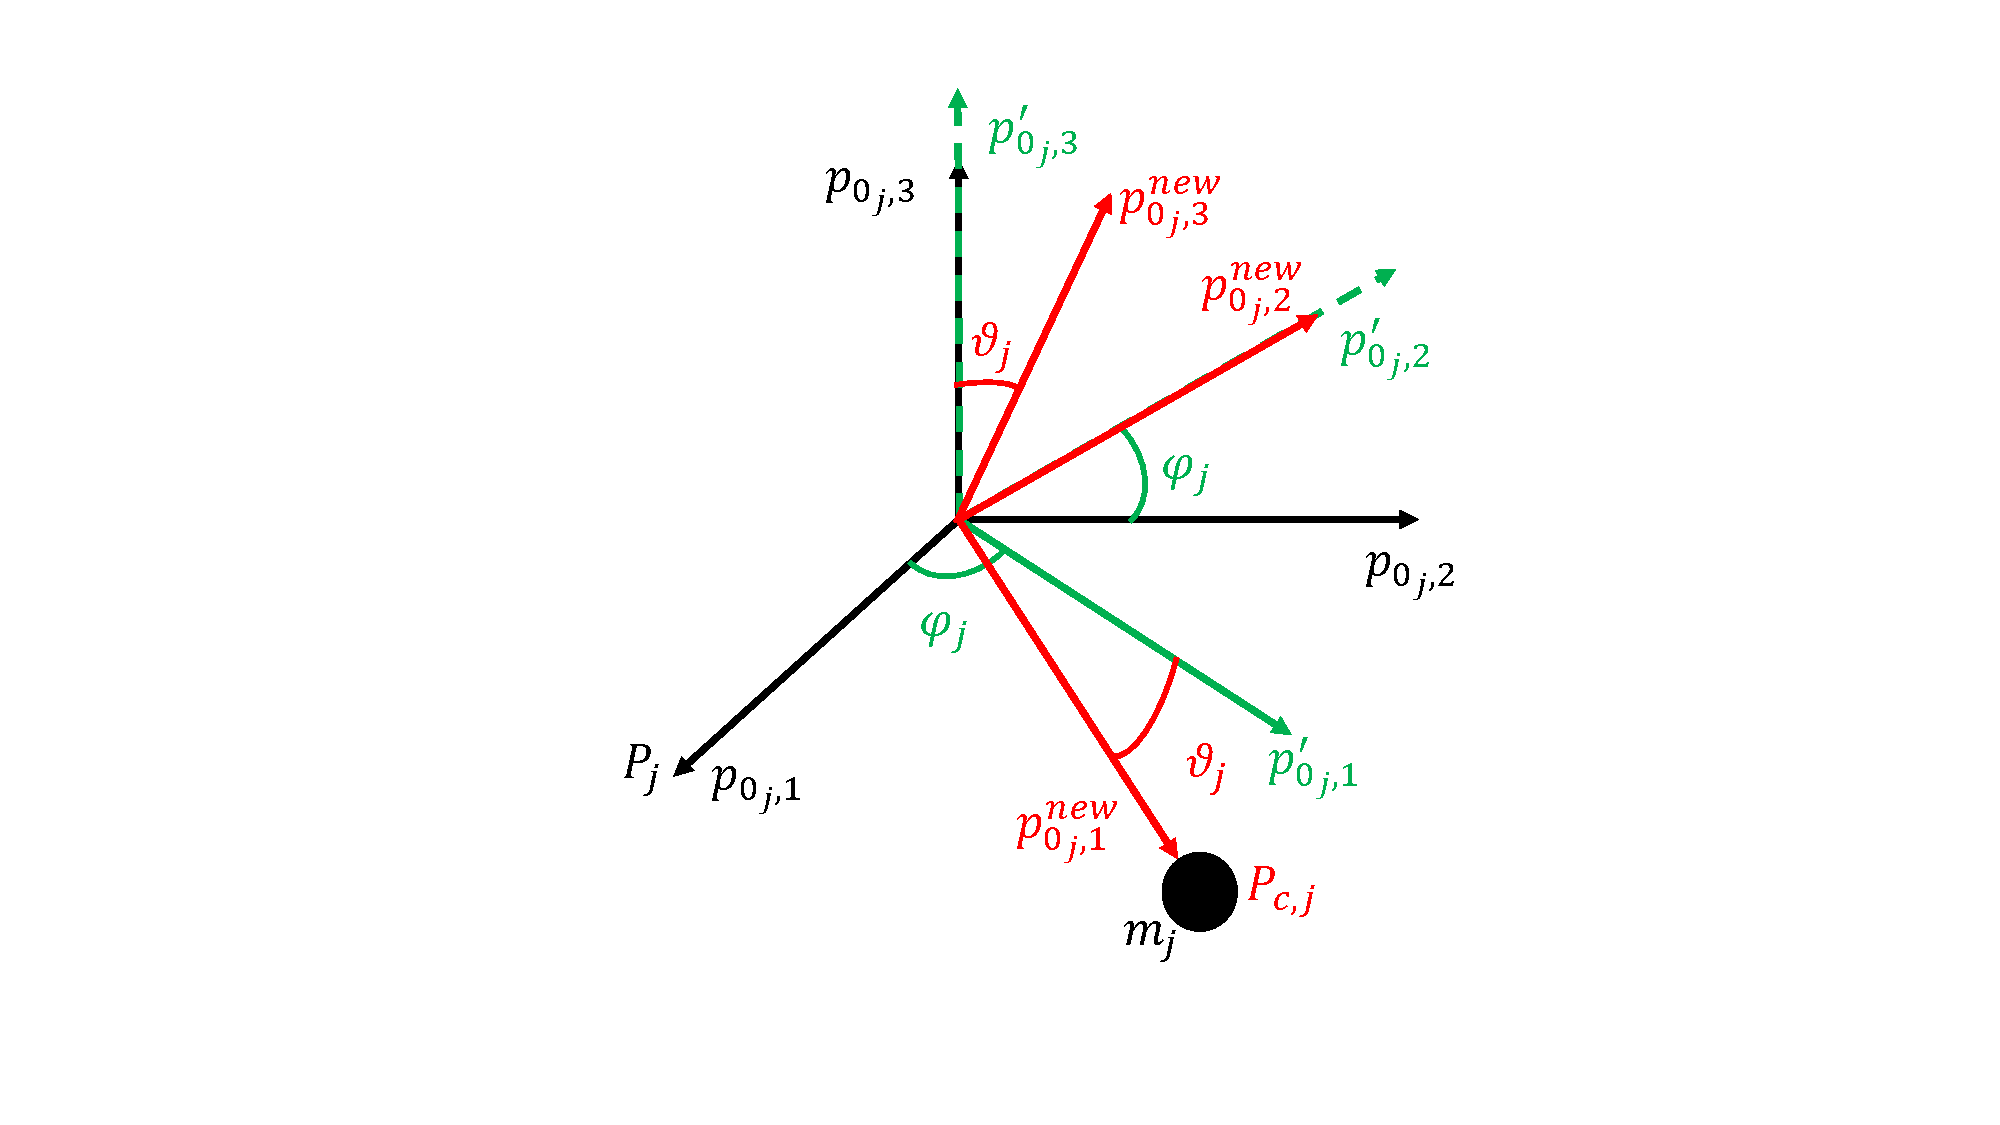
\includegraphics[width=13cm]{Figures/referencesystemsP0.pdf}
	\caption{$\mathcal{P}_{0,j}^{\text{new}}$ frame definition}
	\label{fig:newreferencesystem}
\end{figure} 
At this point is easy to see that the new value of $\varphi_j$ and $\vartheta_j$ are equal to 0. To compute the new value of $\dot{\varphi}_j$ and $\dot{\vartheta}_j$, Eq. \eqref{eq:ljprime} is reversed and it yields:
\begin{equation}
	\dot{\varphi}=\frac{\bm{l}_j[2]}{l_j}
	\label{eq:RSC1}
\end{equation}
\begin{equation}
	\dot{\vartheta}=-\frac{\bm{l}_j[3]}{l_j}
	\label{eq:RSC2}
\end{equation}
The integration can continue using these new values and the new reference systems. This would lead to discontinuities on $\varphi_j$, $\theta_j$, $\varphi_j$ and $\vartheta_j$ but not on the vectors $\bm{l}_j$ and $\bm{l}_{j}'$.